% ---------------------------------------------------------------------------
% Author guideline and sample document for EG publication using LaTeX2e input
% D.Fellner, v1.21, Jan 08, 2024

\documentclass{egpubl}

% Non-EG submissions:
% \usepackage{easyReview}
% \usepackage[hypertexnames=false]{hyperref} 
% \usepackage{geometry}
% \usepackage[inner=1.5cm, outer=5cm]{geometry}
% \usepackage[showframe]{geometry} %just to visualise the borders
% \usepackage{subcaption}

% EG-submissions:
\usepackage{hyperref} 
\ifpdf \usepackage[pdftex]{graphicx} \pdfcompresslevel=9
\else \usepackage[dvips]{graphicx} \fi

% All submissions:
\usepackage[backend=biber, backref=true, backrefstyle=none, style=apa, uniquelist=true, maxcitenames=1, uniquename=false, sortcites=false]{biblatex} 
% \usepackage[utf8]{inputenc}
% \usepackage{mathpazo}
% \usepackage[semibold]{sourcesanspro}
% \usepackage{sectsty}
% \allsectionsfont{\sffamily}
% \usepackage[T1]{fontenc}
% \usepackage[english]{babel}
\usepackage{amsmath} %%%%%%%%%%%%%%%%%%%%%%%
\usepackage{amsfonts} %%%%%%%%%%%%%%%%%%%%%%%
% \usepackage{fancyhdr}
\usepackage{amssymb} %%%%%%%%%%%%%%%%%%%%%%%
% \usepackage{xcolor}
% \definecolor{Valentia}{RGB}{233,78,82}
% \definecolor{Titleblue}{RGB}{114, 146, 162}
% \usepackage{csquotes}
% \usepackage{mdframed}
% \usepackage{multirow} %% Pour mettre un texte sur plusieurs rangées
% \usepackage{multicol} %% Pour mettre un texte sur plusieurs colonnes
% \usepackage{scrextend} % Forcer la 4eme  de couverture en page pair
\usepackage{tikz}
% \usepackage{graphicx}
% \usepackage[absolute]{textpos} 
% \usepackage{colortbl}
% \definecolor{newcolor}{rgb}{.8,.349,.1}
% \usepackage{array}
% \usepackage{microtype}
% \usepackage{framed}
% \usepackage{latexsym}
% \usepackage{url}
% \usepackage[hypcap=false]{caption}
% \usepackage{stackengine}
% \usepackage{svg}
\usepackage{wrapfig}
% \usepackage{pdflscape}
% \usepackage{afterpage}
% \usepackage{capt-of}
% \usepackage{longtable}
% \usepackage{makecell}
% \usepackage{titlesec}
\usepackage{float}
% \usepackage{booktabs}
% \usepackage{tabularx}
\usepackage{siunitx}
%\usepackage{breqn}
% \usepackage{bookmark}
% \usepackage{etoc}
% \usepackage{minitoc}
\usepackage{transparent}
\usepackage[export]{adjustbox}
% \usepackage{etoolbox}
\usepackage{letltxmacro}
% \usepackage{xparse}
\usepackage{listings}
\usepackage{xstring}
% \usepackage{ifthen}
% \usepackage[toc,page]{appendix}
\usepackage[toc, acronym]{glossaries}
% \usepackage{upgreek}
% \usepackage{textgreek}
% \usepackage[minimal=true]{chemmacros}
% \usepackage{indentfirst}
% \usepackage{scalerel}
% \usepackage{stackengine}
% \usepackage{wasysym}
% \usepackage{lscape}
% \usepackage{afterpage}
\usepackage{totcount}
% \usepackage{placeins}
\usepackage{mathtools}
% \usepackage{ragged2e}
\usepackage{enumitem} % for customizing lists
% \usepackage{silence}
% \usepackage{expl3}

% \usepackage[backend=biber, backref=true, backrefstyle=none, style=apa, uniquelist=true, maxcitenames=1, uniquename=false, sortcites=false]{biblatex} 
% backref: add link in the references to go back up
% uniquelist: write "et al." even if the reference can be ambiguous with only first author name
% maxcitenames: Yeah... not sure...
% uniquename: if true and multiple authors have the same last name, the first name initial is added. When dealing with diacritics (accents, cedilles, etc.), it often think that two references have different authors.
% sortcites: when using multi-citations, the sorting is by default an alphabetical order, which has no sense. sortcites=false does not apply sorting, while sortcites=true uses the value of "sorting". If you want to sort by year in the muli-citations but by name in the References section, use "\newrefcontext[sorting=ydnt]" before the text and "\newrefcontext[sorting=nyt]" just before the References section.

% \usepackage{refcheck} % See if some references are missing or if Ids are wrong
\usepackage[capitalise, noabbrev]{cleveref}
\hbadness = 99999

% Non-EG documents:
% \captionsetup{width=\linewidth}


% All documents:


% Define \zzcommand for conditional commands
\def\zzcommand#1{\let#1\undefined\newcommand#1}

% Macros to hold current titles
% \currentsection
\zzcommand{\currentsection}{}
% \currentsubsection
\zzcommand{\currentsubsection}{}
% \currentsubsubsection
\zzcommand{\currentsubsubsection}{}
\makeatletter

% Save original commands
\let\oldsection\section
\let\oldsubsection\subsection
\let\oldsubsubsection\subsubsection

\makeatletter
\gdef\currentsection{}
\gdef\currentsubsection{}
\gdef\currentsubsubsection{}
\zzcommand{\section}[1]{
  \gdef\currentsection{}
  \gdef\currentsubsection{}
  \gdef\currentsubsubsection{}
  \ifthenelse{\equal{#1}{*}}%
  {\@sectionstar}%
  {\@sectionnostar{#1}}%
  % \@ifstar{\@sectionstar}{\@sectionnostar}
}
\zzcommand{\@sectionnostar}[1]{%
  \gdef\currentsection{#1}%
  \oldsection{#1}%
}
\zzcommand{\@sectionstar}[1]{%
  \gdef\currentsection{#1}
  \oldsection*{#1}%
}
\zzcommand{\subsection}[1]{
  \gdef\currentsubsection{}
  \gdef\currentsubsubsection{}
  \ifthenelse{\equal{#1}{*}}%
  {\@subsectionstar}
  {\@subsectionnostar{#1}}
}
\zzcommand{\@subsectionnostar}[1]{%
  \gdef\currentsubsection{#1}%
  \oldsubsection{#1}%
}
\zzcommand{\@subsectionstar}[1]{%
  \gdef\currentsubsection{#1}%
  \oldsubsection*{#1}%
}
\zzcommand{\subsubsection}[1]{
  \gdef\currentsubsubsection{}
  \ifthenelse{\equal{#1}{*}}%
  {\@subsubsectionstar}
  {\@subsubsectionnostar{#1}}
}
\zzcommand{\@subsubsectionnostar}[1]{%
  \gdef\currentsubsubsection{#1}%
  \oldsubsubsection{#1}%
}
\zzcommand{\@subsubsectionstar}[1]{%
  \gdef\currentsubsubsection{#1}%
  \oldsubsubsection*{#1}%
}
\makeatother

% \tensor{expression}
\zzcommand{\tensor}[1]{\mathbf{#1}}
% \mtrx{matrix_name}
\zzcommand{\mtrx}[1]{\mathbf{#1}}
% \field{field_name}
\zzcommand{\field}[1]{\mathbf{#1}}


% \WarningFilter{hyperref}{Token not allowed in a PDF string} % Remove the warnings about \gls in titles or math functions in titles.

\LetLtxMacro{\OldTilde}{\Tilde}
\zzcommand{\Tilde}[1]{
  \StrLen{#1}[\temp]%
  \ifnum\temp>1
    \ThisStyle{%
      \setbox0=\hbox{$\SavedStyle#1$}%
      \stackengine{-.1\LMpt}{$\SavedStyle#1$}{%
        \stretchto{\scaleto{\SavedStyle\mkern.2mu\AC}{.5150\wd0}}{.6\ht0}%
      }{O}{c}{F}{T}{S}%
    }
  \else 
    \OldTilde{#1}
  \fi
}

% \Bar{expression}
\zzcommand{\Bar}[1]{\overline{#1}}


\LetLtxMacro{\Oldincludegraphics}{\includegraphics}
\RenewDocumentCommand{\includegraphics}{O{} m}{%
	\begin{adjustbox}{max width=\linewidth, max height=\textheight-5\baselineskip}
	    \Oldincludegraphics[#1]{#2}
	\end{adjustbox}
}
% \inset{inset_size}{path_to_main_image}{path_to_inset_image}
\zzcommand{\inset}[3][0.2\linewidth]{
    \noindent\stackinset{r}{0.1cm}{b}{0.1cm}{
        \colorbox{white}{
            \includegraphics[width=#1]{#3}
        }
    }
	{\includegraphics{#2}}
}

\let\origfigure\figure
\let\endorigfigure\endfigure

\renewenvironment{figure}[1][tbph]{%
    \origfigure[#1]%
    \centering
}{%
    \endorigfigure
}

% Non-EG submissions:
% % \teaser{/* Inside commands of the figure* environment */}
% \zzcommand{\teaser}[1]{
%     \begin{figure*}[ht]
%         \centering
%         #1
%     \end{figure*}
% }

% \minitoc
\def\minitoc{
	\etocsettocstyle{\section*{\contentsname}}{}
	\localtableofcontents
	\noindent\textbf{\hyperlink{tocpage}{$\uparrow$ Back to summary}}
}
% \makeatletter\@addtoreset{chapter}{part}\makeatother%

\sisetup{product-units=repeat}

\emergencystretch=1em

\zzcommand{\cellalign}{cl}
\newcolumntype{H}{>{\setbox0=\hbox\bgroup}c<{\egroup}@{}}

% Non-EG submissions:
% \DeclareCiteCommand{\cite}[\mkbibparens]
%   {\usebibmacro{prenote}\usebibmacro{cite:init}}%
%   {\usebibmacro{citeindex}\usebibmacro{countcite}{\thefield{entrykey}}%
%   \printtext[bibhyperref]{\usebibmacro{cite}}}%
%   {\multicitedelim}%
%   {\usebibmacro{postnote}}

% \newbibmacro*{citefullbody}{%
%   \printnames{labelname}%
%   \setunit{\addcomma\space}%
%   \textit{\printfield[]{title}}~(\printfield{year})%
% }

% \DeclareCiteCommand{\citep}
% {\usebibmacro{prenote}\usebibmacro{cite:init}}%
% {\usebibmacro{citeindex}\usebibmacro{countcite}{\thefield{entrykey}}%
% \printtext[bibhyperref]{\usebibmacro{citefullbody}}}%
% {\multicitedelim}%
% {\usebibmacro{postnote}}


% \DeclareCiteCommand{\citeProgram}[\mkbibparens]
%   {\usebibmacro{prenote}\usebibmacro{cite:init}}
%   {\usebibmacro{citeindex}\usebibmacro{countcite}{\thefield{entrykey}}\printtext[bibhyperref]{\mkbibemph{\printfield{title}},~\printdate}}
%   {\multicitedelim}
%   {\usebibmacro{postnote}}

% \AtEveryBibitem{\clearfield{url}}
% \AtEveryBibitem{\clearfield{doi}}
% \AtEveryBibitem{\clearfield{note}} % Notes from Mendeley
% \newtotcounter{citenum}
% \AtEveryBibitem{\stepcounter{citenum}}


% \renewbibmacro*{title}{%
% {}
% {\printtext[title]{\mkbibbold{\printfield[title]{title}}}\newunit}}

% \DefineBibliographyStrings{english}{
%   backrefpage = {Cited on page},
%   backrefpages = {Cited on pages},
% }
% \setlength\bibitemsep{1.2\itemsep}

\newcounter{AltTextImageCurrentSide}

% \begin{Itemize}
%     \Item{$1} $2
% \end{Itemize}
% \length{\parindent}{0}
\newenvironment{Itemize}
{    
  \setcounter{AltTextImageCurrentSide}{0}
  \begin{itemize}[label={}, leftmargin=\parindent, itemindent=1.0em, itemsep=0em, topsep=0em] %, left=2em, itemsep=0.5em]} % Custom settings
}
{\end{itemize}\bigbreak}

% Define new command \Itemthat applies italics to the title only
% \Item{text}
\zzcommand{\Item}[1]{%
  \ifblank{#1}%
    {\item $\bullet$ }% Case when #1 is empty
    {\item \textit{#1}}% Case when #1 is not empty
}

\newlength{\currentparindent}
\newlength{\contentheightofalttextimage}
\newsavebox{\alttextbox}



% Non-EG Only:
% \ExplSyntaxOn
% % \AltTextImageR{item_content}{placeholder.pdf}{caption}{label}
% \zzcommand{\AltTextImageR}[4]{% 
%   \setcounter{AltTextImageCurrentSide}{1}
%   \setlength{\currentparindent}{\parindent}%
%   % \newsavebox{\alttextbox}
%     \sbox{\alttextbox}{\vbox{\hsize=0.65\linewidth #1}}%
%     \setlength{\contentheightofalttextimage}{\ht\alttextbox}%
%   \noindent
%   \begin{minipage}[t]{0.65\linewidth}
%     \setlength{\parindent}{\currentparindent}
%     #1
%   \end{minipage}%
%   \hfill % Add horizontal space between text and image
%   \begin{minipage}[t]{0.30\linewidth}    
%     \centering
%     % Parse comma-separated images and stack them
%     \seq_set_split:Nnn \l_tmpa_seq { , } { #2 }%
%     \int_set:Nn \l_tmpa_int { \seq_count:N \l_tmpa_seq }%
%     \dim_set:Nn \l_tmpa_dim { \contentheightofalttextimage / \l_tmpa_int }%
%     \seq_map_inline:Nn \l_tmpa_seq {%
%       \includegraphics[width=\linewidth, height=\l_tmpa_dim, keepaspectratio, valign=t]{##1}\\%
%     }%
%     % \includegraphics[width=\linewidth, height=\contentheightofalttextimage, keepaspectratio, valign=t]{#2}
%     \captionsetup{font=footnotesize} %%%%%%%%%%%%%%%%%%%%%%%%%%%%%%%%%%%%%%%
%     \captionsetup{width=\linewidth} %%%%%%%%%%%%%%%%%%%%%%%%%%%%%%%%%%%%%%%
%     \captionof{figure}{#3} %%%%%%%%%%%%%%%%%%%%%%%%%%%%%%%%%%%%%%%
%     % \caption{#3}
%     \label{#4}
%   \end{minipage}%
% }
% % \AltTextImageL{item_content}{placeholder.pdf}{caption}{label}
% \zzcommand{\AltTextImageL}[4]{% 
%   \setcounter{AltTextImageCurrentSide}{0}
%   \setlength{\currentparindent}{\parindent}%
%     \sbox{\alttextbox}{\vbox{\hsize=0.65\linewidth #1}}%
%     \setlength{\contentheightofalttextimage}{\ht\alttextbox}%
%   \noindent
%   \begin{minipage}[t]{0.30\linewidth}
%     \centering
%     % Parse comma-separated images and stack them
%     \seq_set_split:Nnn \l_tmpa_seq { , } { #2 }%
%     \int_set:Nn \l_tmpa_int { \seq_count:N \l_tmpa_seq }%
%     \dim_set:Nn \l_tmpa_dim { \contentheightofalttextimage / \l_tmpa_int }%
%     \seq_map_inline:Nn \l_tmpa_seq {%
%       \includegraphics[width=\linewidth, height=\l_tmpa_dim, keepaspectratio, valign=t]{##1}\\%
%     }%
%     % \includegraphics[width=\linewidth, height=\contentheightofalttextimage, keepaspectratio, valign=t]{#2}
%     \captionsetup{font=footnotesize} %%%%%%%%%%%%%%%%%%%%%%%%%%%%%%%%%%%%%%%
%     \captionsetup{width=\linewidth} %%%%%%%%%%%%%%%%%%%%%%%%%%%%%%%%%%%%%%%
%     \captionof{figure}{#3} %%%%%%%%%%%%%%%%%%%%%%%%%%%%%%%%%%%%%%%
%     % \caption{#3}
%     \label{#4}
%   \end{minipage}%
%   \hfill % Add horizontal space between text and image
%   \begin{minipage}[t]{0.65\linewidth}
%     \setlength{\parindent}{\currentparindent}
%     #1
%   \end{minipage}%
% }
% \ExplSyntaxOff


% EG only:
\ExplSyntaxOn
% \AltTextImageR{item_content}{placeholder.pdf}{caption}{label}
\zzcommand{\AltTextImageR}[4]{% 
  \setcounter{AltTextImageCurrentSide}{1}%
    #1%
  \begin{figure}[tbh]%
    \centering%
    % Parse comma-separated images and stack them
    \seq_set_split:Nnn \l_tmpa_seq { , } { #2 }%
    \int_set:Nn \l_tmpa_int { \seq_count:N \l_tmpa_seq }%
    \dim_set:Nn \l_tmpa_dim { \contentheightofalttextimage / \l_tmpa_int }%
    \seq_map_inline:Nn \l_tmpa_seq {%
      \includegraphics[width=\linewidth]{##1}%
    }%
    \caption{#3}%
    \label{#4}%
  \end{figure}%
}
% \AltTextImageL{item_content}{placeholder.pdf}{caption}{label}
\zzcommand{\AltTextImageL}[4]{% 
  \AltTextImageR{#1}{#2}{#3}{#4}%
}
\ExplSyntaxOff























% \AltTextImage{item_content}{placeholder.pdf}{caption}{label}
\zzcommand{\AltTextImage}[4]
{
  \stepcounter{AltTextImageCurrentSide}  % Increment the counter
  \ifodd\value{AltTextImageCurrentSide}  % Check if the counter is odd
      \AltTextImageR{#1}{#2}{#3}{#4}
  \else%
      \AltTextImageL{#1}{#2}{#3}{#4}
  \fi
}
\ExplSyntaxOff

% \AltTextImage{item_content}{placeholder.pdf}{caption}{label}
\zzcommand{\AltTextImage}[4]
{
  \stepcounter{AltTextImageCurrentSide}  % Increment the counter
  \ifodd\value{AltTextImageCurrentSide}  % Check if the counter is odd
      \AltTextImageR{#1}{#2}{#3}{#4}
  \else%
      \AltTextImageL{#1}{#2}{#3}{#4}
  \fi
}

\lstset {
    language=C++,
    backgroundcolor=\color{black!5}, % set backgroundcolor
    basicstyle=\footnotesize,% basic font setting
}

\makeglossaries
\DeclareDocumentCommand{\newdualentry}{ O{} O{} m m m m g } {
    \newglossaryentry{gls-#3}{
        name={#5},
        text={#5\if\relax\detokenize{#4}\relax\else\glsadd{#3}\fi},
        plural={\IfValueTF{#7}{#7}{#5s}},
        longplural={\IfValueTF{#7}{#7}{#5s}},
        description={#6},
        #1
    }
    \if\relax\detokenize{#4}\relax
    % nothing
  \else
    \newacronym[longplural={\IfValueTF{#7}{#7}{#5s}}, 
        see={[Glossary:]{gls-#3}},
        #2]{#3}{#4}{#5\glsadd{gls-#3}}
  \fi
    \makeglossaries
}


% \gloss{entry_name}
\zzcommand{\gloss}[1]{\ifglsentryexists{gls-#1}{\glsentryname{gls-#1}\ifcsdef{inheading}{}{{\glsadd{gls-#1}}}}{[XXXX]}}
% \glosses{entry_name}
\zzcommand{\glosses}[1]{\ifglsentryexists{gls-#1}{\glsentrylongpl{gls-#1}\ifcsdef{inheading}{}{{\glsadd{gls-#1}}}}{[XXXX]}}
% \Gloss{entry_name}
\zzcommand{\Gloss}[1]{\ifglsentryexists{gls-#1}{\Glsentryname{gls-#1}\ifcsdef{inheading}{}{{\glsadd{gls-#1}}}}{[XXXX]}}
% \Glosses{entry_name}
\zzcommand{\Glosses}[1]{\ifglsentryexists{gls-#1}{\Glsentrylongpl{gls-#1}\ifcsdef{inheading}{}{{\glsadd{gls-#1}}}}{[XXXX]}}
\zzcommand{\glsnamefont}[1]{\makefirstuc{#1}}

% \eqref{label}
\zzcommand{\eqref}[1]{\cref{#1}}
% \to 
\zzcommand{\to}{\mapsto}


% \subsubsubsection{title}
\zzcommand{\subsubsubsection}[1]{\bigskip\noindent\textit{#1}\nopagebreak\par}
% \subsubsubsubsection{title}
\zzcommand{\subsubsubsubsection}[1]{\bigskip\noindent\textbf{#1}~}

% \wrapFig{img_path}{width}{label}{caption}
\zzcommand{\wrapFig}[4]{
  \wrapFigL{#1}{#2}{#3}{#4}
}

\newlength{\prevColumnsep}
% \wrapFigLR{img_path}{width}{label}{caption}{|L,R|}
\zzcommand{\wrapFigLR}[5]{
  % \begingroup
  % \setlength{\prevColumnsep}{\columnsep}
  \setlength{\columnsep}{1em}
  \def\tempwidth{#2}%
  \ifx\tempwidth\empty
    \def\tempwidth{0.25}%
  \fi
  \begin{wrapfigure}{#5}{\tempwidth \linewidth}
    \centering
    \includegraphics[width=\linewidth]{#1}
    \expandafter\ifx\expandafter\relax\detokenize{#4}\relax\else\caption{#4}\fi
    \expandafter\ifx\expandafter\relax\detokenize{#3}\relax\else\label{#3}\fi
    % \vspace{-1 \baselineskip}
  \end{wrapfigure}
  % \setlength{\columnsep}{\prevColumnsep}
  % \endgroup
}

% \wrapFigL{img_path}{width}{label}{caption}
\zzcommand{\wrapFigL}[4]{
  \wrapFigLR{#1}{#2}{#3}{#4}{L}
}
% \wrapFigR{img_path}{width}{label}{caption}
\zzcommand{\wrapFigR}[4]{
  \wrapFigLR{#1}{#2}{#3}{#4}{R}
}

% \zzcommand{\abstract}
% {
%     \section*{Abstract}
% }

% % \shortAbstract{text}
% \zzcommand{\shortAbstract}[1]
% {
%   \noindent
%   \textit{#1}
%   \bigskip
% }

\zzcommand{\smallConclusion}
{
  \bigskip
}
  
\zzcommand{\midConclusion}
{
  \bigskip\bigskip\bigskip
}

\ExplSyntaxOn
\NewDocumentCommand{\appendtographicspath}{m}
 {
  \tl_if_exist:cF { Ginput@path } { \tl_new:c { Ginput@path } }
  \tl_gput_right:cn {Ginput@path} { #1 }
 }
\NewDocumentCommand{\prependtographicspath}{m}
 {
  \tl_if_exist:cF { Ginput@path } { \tl_new:c { Ginput@path } }
  \tl_gput_left:cn {Ginput@path} { #1 }
 }
\ExplSyntaxOff

% \resetgraphicspath
\zzcommand{\resetgraphicspath}
{
  \graphicspath{}
}

% \hide{text}
\zzcommand{\hide}[1] {}




% Counter for citations per section
\newcounter{sectioncites}
\newcounter{subsectioncites}
\newcounter{subsubsectioncites}

% Macro to store list of citation keys used in current section
\zzcommand{\sectioncitedkeyslist}{,} % Start with a leading comma
\zzcommand{\subsectioncitedkeyslist}{,} % Start with a leading comma
\zzcommand{\subsubsectioncitedkeyslist}{,} % Start with a leading comma

% Reset at each section
\zzcommand{\resetsectioncites}{%
  \setcounter{sectioncites}{0}%
  \zzcommand{\sectioncitedkeyslist}{,}%
  \resetsubsectioncites
}
\zzcommand{\resetsubsectioncites}{%
  \setcounter{subsectioncites}{0}%
  \zzcommand{\subsectioncitedkeyslist}{,}%
  \resetsubsubsectioncites
}
\zzcommand{\resetsubsubsectioncites}{%
  \setcounter{subsubsectioncites}{0}%
  \zzcommand{\subsubsectioncitedkeyslist}{,}%
}
% Helper: checks if key is in the list, and adds if not
\zzcommand{\adduniquecite}[1]{%
  \def\currentkey{#1}%
  \IfSubStr{\sectioncitedkeyslist}{,\currentkey,}{\def\foundkey{1}}{\def\foundkey{0}}%
  \ifnum\foundkey=0%
    \stepcounter{sectioncites}%
    \xappto{\sectioncitedkeyslist}{,\currentkey,}%
  \fi%
  \IfSubStr{\subsectioncitedkeyslist}{,\currentkey,}{\def\foundkey{1}}{\def\foundkey{0}}%
  \ifnum\foundkey=0%
    \stepcounter{subsectioncites}%
    \xappto{\subsectioncitedkeyslist}{,\currentkey,}%
  \fi%
  \IfSubStr{\subsubsectioncitedkeyslist}{,\currentkey,}{\def\foundkey{1}}{\def\foundkey{0}}%
  \ifnum\foundkey=0%
    \stepcounter{subsubsectioncites}%
    \xappto{\subsubsectioncitedkeyslist}{,\currentkey,}%
  \fi%
}

% Custom bibmacro to do the tracking per entry
\newbibmacro*{countcite}[1]{%
  \adduniquecite{#1}%
}
\zzcommand{\showsectioncites}{%
  \notblank{\currentsection}{%
  \ifdef{\thesectioncites}{%
    \ifnum\thesectioncites=0%
    \else%
      \textcolor{white}{\texttransparent{0.0}{~\thesectioncites~(\currentsection)}}%
    \fi%
  }{}}{}%
}
\zzcommand{\showsubsectioncites}{%
  \notblank{\currentsubsection}{%
  \ifdef{\thesubsectioncites}{%
    \ifnum\thesubsectioncites=0%
    \else%
      \textcolor{white}{\texttransparent{0.0}{~\thesubsectioncites~(\currentsubsection)}}%
    \fi%
  }{}}{}%
}
\zzcommand{\showsubsubsectioncites}{%
  \notblank{\currentsubsubsection}{%
  \ifdef{\thesubsubsectioncites}{%
    \ifnum\thesubsubsectioncites=0%
    \else%
      \textcolor{white}{\texttransparent{0.0}{~\thesubsubsectioncites~(\currentsubsubsection)}}%
    \fi%
  }{}}{}%
}

\pretocmd{\section}{\showsubsubsectioncites\showsubsectioncites\showsectioncites\resetsectioncites}{}{}
\pretocmd{\subsection}{\showsubsubsectioncites\showsubsectioncites\resetsubsectioncites}{}{}
\pretocmd{\subsubsection}{\showsubsubsectioncites\resetsubsubsectioncites}{}{}









% === User-facing macro ===
% Holds user-defined row width
\newcommand{\fitrowwidth}{\linewidth}
\newcommand{\fitimageoptions}{}

% autofitgraphics with [options]{img1,img2,...}
\makeatletter
\NewDocumentCommand{\autofitgraphics}{O{} m}{%
  \renewcommand{\fitrowwidth}{\linewidth}%
  \def\fitimageoptions{}%
  \def\cleanopts{}%

  \def\tempa{#1}%
  \@for\opt:=\tempa\do{%
    \IfBeginWith{\opt}{width=}%
      {\StrBehind{\opt}{=}[{\tempwidth}]\renewcommand{\fitrowwidth}{\tempwidth}}%
      {\ifx\cleanopts\@empty
         \edef\cleanopts{\opt}%
       \else
         \edef\cleanopts{\cleanopts,\opt}%
       \fi
      }%
  }%
  \edef\fitimageoptions{\cleanopts}%
  \fitNimages{#2}%
}
\makeatother

\newcounter{fitImgCount}%
\newcounter{fitImgIndex}%
\newcommand{\fitNimages}[1]{%
  \setcounter{fitImgCount}{0}
  \setcounter{fitImgIndex}{0}
  \begingroup
  
  \def\fitTotalRatio{0}%
  \global\let\fitWidths\empty
  \def\fitImgList{}%

  % Copy input to a clean list for repeated processing
  \renewcommand{\do}[1]{%
    \edef\fitImgList{\fitImgList,##1}%
  }%
  \docsvlist{#1}%

  % First pass: calculate total aspect ratio and store individual ratios
  \renewcommand{\do}[1]{%
    \stepcounter{fitImgCount}%
    \sbox0{\includegraphics{##1}}%
    \edef\imgWidth{\the\wd0}%
    \edef\imgHeight{\the\ht0}%
    \pgfmathsetmacro{\imgRatio}{\imgWidth/\imgHeight}%
    \pgfmathparse{\fitTotalRatio + \imgRatio}%
    \xdef\fitTotalRatio{\pgfmathresult}%
    \expandafter\xdef\csname fitRatio\thefitImgCount\endcsname{\imgRatio}%
  }%
  \docsvlist{#1}%

  % Second pass: output images with proportional widths
  \setcounter{fitImgIndex}{0}%
  \begin{adjustbox}{width=\fitrowwidth}%
  \renewcommand{\do}[1]{%
    \stepcounter{fitImgIndex}%
    \pgfmathsetmacro{\relwidth}{\csname fitRatio\thefitImgIndex\endcsname / \fitTotalRatio}%
    \xdef\fitWidth{\relwidth}%
    \expandafter\xdef\csname fitWidth\thefitImgIndex\endcsname{\fitWidth}%
    \expandafter\includegraphics\expandafter[\fitimageoptions, width=\fitWidth\linewidth]{##1}%

  }%
  \docsvlist{#1}%
  \end{adjustbox}%
  \endgroup
}
\newcounter{fitCapIndex}
\NewDocumentCommand{\autofitcaptions}{O{2ex} m}{%
  \setcounter{fitCapIndex}{0}%
  \begin{adjustbox}{width=\fitrowwidth}%
  \renewcommand{\do}[1]{%
    \stepcounter{fitCapIndex}%
    \pgfmathsetmacro{\relwidth}{\csname fitRatio\thefitCapIndex\endcsname / \fitTotalRatio}%
    \raisebox{#1}{\parbox[t]{\relwidth\linewidth}{\centering ##1}}%
    }%
    \docsvlist{#2}%
  \end{adjustbox}%
  \vspace{-#1}\vspace{-#1}
}




% \delete{text_to_remove}
\zzcommand{\delete}[1]
{\remove{#1}}
\zzcommand{\comment}[1]
{\par \highlight{~!~!~!~!~!~!~!~!~!~!~} #1 \highlight{~!~!~!~!~!~!~!~!~!~!~} \\}
\zzcommand{\Replace}{\replace}
\zzcommand{\Comment}{\comment}
\zzcommand{\Add}{\add}
\zzcommand{\Delete}{\delete}
\zzcommand{\revrepl}{\replace}
\zzcommand{\revnote}{\comment}


\makeatletter
% define a macro to collect figure content
\newcommand{\deferredfloats}{}

% define an environment that stores the full content for later use
\newenvironment{deferredfigure}
  {\collect@body\storedeferredfigure}
  {}

\newcommand{\storedeferredfigure}[1]{%
  \gappto\deferredfloats{%
    \begin{figure}[htbp]
    #1
    \end{figure}
  }%
}
\makeatother

\zzcommand{\paragraph}[1]{\noindent\textbf{#1}\ }

% \floor{x}
\zzcommand{\floor}[1]{\lfloor#1\rfloor}
% \ceil{x}
\zzcommand{\ceil}[1]{\lceil#1\rceil}
\zzcommand{\R}{\mathbb{R}}
\zzcommand{\N}{\mathbb{N}}
\zzcommand{\C}{\mathbb{C}}
\zzcommand{\Z}{\mathbb{Z}}
% \norm{vec}
\zzcommand{\norm}[1]{\left\lVert #1 \right\rVert}
% \abs{x}
\zzcommand{\abs}[1]{\left| #1 \right|}

\zzcommand{\obj}{\text{STE}}

\zzcommand{\material}{\mathcal{M}}

\zzcommand{\mass}{m}
\zzcommand{\velFactor}{\nu}
\zzcommand{\decay}{k}
\zzcommand{\diffusion}{D}
\zzcommand{\growthRate}{\gamma}
\zzcommand{\fitnessFunc}{\omega}
\zzcommand{\fitnessFuncObj}{\fitnessFunc_\obj}
\zzcommand{\fittingFunc}{\Gamma}
\zzcommand{\fittingFuncObj}{\fittingFunc_\obj}

\zzcommand{\Water}{\mathcal{W}}
\zzcommand{\Wuser}{\Water_\text{user}}
\zzcommand{\Wsimu}{\Water_\text{simulation}}
\zzcommand{\Wobj}{\waterModif_\text{objects}}

\zzcommand{\terrain}{\mathcal{T}}
\zzcommand{\height}{\mathcal{H}}
\zzcommand{\depth}{\mathcal{D}}
\zzcommand{\objects}{\mathcal{O}}
\zzcommand{\environment}{\mathcal{E}}
\zzcommand{\Wlevel}{\mathcal{L}}
\zzcommand{\events}{\text{events}}

\zzcommand{\groundedHeight}{\mathcal{G}}
\zzcommand{\altitudeHeight}{\mathcal{A}}
\zzcommand{\surfaceHeight}{\mathcal{S}}

\zzcommand{\availableObjects}{\Tilde{\objects}}
\zzcommand{\targetObjects}{\Hat{\objects}}

\zzcommand{\environmentModif}{\environment^+}
\zzcommand{\heightModif}{\height^+}
\zzcommand{\waterModif}{\Water^+}
\zzcommand{\materialModif}{\material^+}
\zzcommand{\nothing}{\emptyset}

\zzcommand{\tEvent}{t_e}

\zzcommand{\eps}{\varepsilon}


\zzcommand{\erosionRate}{ \varepsilon }
\zzcommand{\shearStress}{ \tau }
\zzcommand{\shearRate}{\theta}
\zzcommand{\criticalShearStress}{ \shearStress_\text{critical} }
\zzcommand{\velocity}{ \upsilon }
\zzcommand{\capacity}{ C }
\zzcommand{\maxCapacity}{ \capacity_\text{max} }
\zzcommand{\density}{ \rho }
\zzcommand{\particleDensity}{ \density_\text{particle} }
\zzcommand{\soilDensity}{ \density_\text{sediment} }
\zzcommand{\particleMass}{ \mass_\text{particle} }
\zzcommand{\depositionRate}{ \omega } % Not the good notation, but I don't think there is a real notation
\zzcommand{\shearStressConstant}{ K }
\zzcommand{\erosionStrength}{ K_{\erosionRate} }
\zzcommand{\particleSize}{ R }
\zzcommand{\settlingVelocity}{ w_s }
\zzcommand{\fluid}{ \text{fluid} }
\zzcommand{\fluidDensity}{ \density_\fluid }
\zzcommand{\fluidVelocity}{ \velocity_\fluid }
\zzcommand{\erosionAmount}{ q_\text{detachment} }
\zzcommand{\depositAmount}{ q_\text{deposit} }
\zzcommand{\totalErosion}{ Q }
\zzcommand{\extForce}{ \vec F_\text{ext} }
\zzcommand{\capacityFactor}{ C_\text{factor} }


\zzcommand{\area}{a}
\zzcommand{\Area}{A}
\zzcommand{\length}{l}
\zzcommand{\Length}{L}
\zzcommand{\energy}{E}
\zzcommand{\Einternal}{\energy_{\text{internal}}}
\zzcommand{\Eexternal}{\energy_{\text{external}}}
\zzcommand{\Eshape}{\energy_{\text{shape}}}
\zzcommand{\Esnake}{\energy_{\text{snake}}}
\zzcommand{\Econt}{\energy_{\text{continuity}}}
\zzcommand{\Eimage}{\energy_{\text{image}}}
\zzcommand{\Ecurv}{\energy_{\text{curvature}}}
\zzcommand{\Egradient}{\energy_{\text{gradient}}}

\zzcommand{\Ainternal}{\alpha_{\text{i}}}
\zzcommand{\Aexternal}{\alpha_{\text{e}}}
\zzcommand{\Ashape}{\alpha_{\text{s}}}
\zzcommand{\Acont}{\alpha_{\text{c}}}
\zzcommand{\Aimage}{\alpha_{\text{i}}}
\zzcommand{\Acurv}{\alpha_{\text{c}}}
\zzcommand{\Agradient}{\alpha_{\text{g}}}

% \zzcommand{\time}{t}
\zzcommand{\curve}{C}
\zzcommand{\absorption}{A}
\zzcommand{\deposition}{D}
\zzcommand{\p}{\tensor{p}}
\zzcommand{\q}{\tensor{q}}
\zzcommand{\domain}{\Omega}
\zzcommand{\warp}{\Phi}
\zzcommand{\force}{\mtrx{F}}
\zzcommand{\influence}{\lambda}
\zzcommand{\windVelocity}{\velocity_{\text{wind}}}
\zzcommand{\std}{\sigma}
\zzcommand{\temperature}{T}
\zzcommand{\dirac}{\delta}
\zzcommand{\identity}{\mtrx{I}}

\zzcommand{\heightmap}{H}
\zzcommand{\implicit}{I}
\zzcommand{\densityVox}{DV}
\zzcommand{\binaryVox}{BV}

\zzcommand{\volume}{V}
\zzcommand{\gravity}{\vec g}
\zzcommand{\gravityForce}{\vec F_{\text{gravity}}}
\zzcommand{\buoyancyForce}{\vec F_{\text{buoyancy}}}
\zzcommand{\constGravity}{G}
\zzcommand{\viscosity}{\mu}

\zzcommand{\radius}{r}
\zzcommand{\Radius}{R}

\zzcommand{\noise}{\eta}

% \dot{vecA}{vecB}
\zzcommand{\dot}[2]{\langle  #1  , #2 \rangle}


\zzcommand{\lerp}{\operatorname{lerp}}
\zzcommand{\smooth}{\operatorname{smoothstep}}
\zzcommand{\smoothmin}{\operatorname{smin}}
\zzcommand{\smoothmax}{\operatorname{smax}}
\zzcommand{\sigmoid}{\operatorname{sigmoid}}

\zzcommand{\heightProfile}{h_{\text{profile}}}
\zzcommand{\heightSubsid}{h_{\text{subsid}}}
\zzcommand{\heightCoral}{h_{\text{coral}}}
\zzcommand{\coralMin}{z_\text{coral min}}
\zzcommand{\coralMax}{z_\text{coral max}}
\zzcommand{\resistance}{\rho}
\zzcommand{\subsidRate}{\lambda}
\zzcommand{\distRegions}{\Tilde{x}}

\zzcommand{\angl}{\theta}
\zzcommand{\anglTwo}{\phi}
% \closest{curve}{point}
\zzcommand{\closest}[2]{{#2}^{*}_{#1}}
% \closestC{point}
\zzcommand{\closestC}[1]{\closest{\curve}{#1}}
\zzcommand{\closestCp}{\closest{\curve}{\p}}

% \newdualentry[glossary-options][abbrev. options]{key}{abbr}{Full name}{Description}{Plural (opt)}
%Intro
\newdualentry[][]{ParamSpace}{}{parameter space}{Set of adjustable parameters that can be modified to control and influence the generation process of content or assets. These parameters can include properties like size, shape, density, or other relevant factors, depending on the specific procedural algorithm being used. By adjusting these parameters, creators can achieve a wide variety of outcomes and patterns, enabling the generation of diverse and customizable content such as textures, levels, or 3D models.}
\newdualentry[][]{LOD}{LoD}{level of detail}{Amount of graphical data or information displayed in a scene or image. Higher LOD means more detail, while lower LOD means less detail. This concept helps manage computational resources, where less important or distant objects have lower LOD to improve performance.}

% Semantic
\newdualentry[][]{EnvObj}{}{environmental object}{Geographic feature represented sparsly which describe a landscape. We represent it with a \gloss{Skeleton}, \glosses{GenRule} and \glosses{EnvMat}. }
\newdualentry[][]{EnvVal}{}{environmental attribute}{Value of a geographic field at one point in space and time. }
\newdualentry[][]{EnvModif}{}{environmental modifier}{Description of a modification of a \gloss{EnvVal} around a \gloss{EnvObj}. It can represent the spread or the absorption of material around it, or the deformation of water currents. }
\newdualentry[][]{EnvMat}{}{environmental material}{Material available.}
\newdualentry[][]{GeoEvent}{}{geomorphic event}{Modification of a \gloss{EnvVal} in an interval of time with or without spatial bounds. }
\newdualentry[][]{Skeleton}{}{skeleton}{Simplified shape of a \gloss{EnvObj}, as it could be symbolized in a map: as a point, a curve or a region. }
\newdualentry[][]{GenRule}{}{generation rule}{Composed of a \gloss{FitnessFunc} and \gloss{FittingFunc}, the optimisation of the \gloss{GenRule} of an \gloss{EnvObj} through the maximization of its components describe where and how new elements can be added to a semantic terrain. }
\newdualentry[][]{FitnessFunc}{}{fitness function}{Function affected to a \gloss{EnvObj} that, given the \gloss{EnvVal} at a $(x, y)$ position in the space, returns a score describing how well this \gloss{EnvObj} may survive. }
\newdualentry[][]{FittingFunc}{}{skeleton fitting function}{Function affected to a \gloss{EnvObj} that, given the local \gloss{EnvVal} and the shape of the skeleton of the \gloss{EnvObj}, returns a score describing how well this \gloss{EnvObj} fits. It may be seen as a refinement of the \gloss{FitnessFunc}. }
\newdualentry[][]{SteadyState}{}{steady state}{A system is at steady state when internal properties do not change overtime once a dynamic equilibrium has been reached. The \glosses{EnvMat} emission from \glosses{EnvObj} can be seen as a thermodynamic system which achieve thermodynamic equilibrium over time. }
\newdualentry[][]{CoarseHeight}{}{coarse height function}{Simplified function representing the height of a \gloss{EnvObj} in the 2D plane, useful to estimate the altitude of a point $\p$ of the terrain $\height(\p)$ as a combination of the \gloss{CoarseHeight} of all \glosses{EnvObj} close to $\p$. }





\newdualentry[][]{WarpFunction}{}{warp function}{$\warp: \R^n \to \R^n$ is a function that, given a $n$-dimensional point $\p$ returns another point $\q$. The function is usually bijective.}

% Introduction
\newdualentry[][]{ProceduralGeneration}{}{procedural generation}{A method for creating data algorithmically rather than manually, used across various fields to automate content creation.}
\newdualentry[][]{TerrainGeneration}{}{terrain generation}{The process of algorithmically creating landforms in virtual environments, often using mathematical models and noise functions to simulate natural terrains.}
\newdualentry[][]{VirtualTerrain}{}{virtual terrain}{Digitally simulated landscape used in video games, simulations, and visualizations, which mimics real-world or imaginary terrains.}
\newdualentry[][]{ComputerGraphics}{}{computer graphics}{The field of computing dedicated to generating and managing visual content and images through software and hardware.}
\newdualentry[][]{Seascape}{}{seascape}{An underwater environment or ecosystem, important in marine biology and underwater photography.}
\newdualentry[][]{TerrainRepresentation}{}{terrain representation}{Different methods used to depict geographical features in two-dimensional and three-dimensional formats.}
\newdualentry[][]{FluidSimulation}{}{fluid simulation}{A computational method to model fluid behaviors in graphics, gaming, and simulation, often using algorithms that calculate the motion and interaction of liquids and gases.}
\newdualentry[][]{FluidSolver}{}{fluid solver}{A software or algorithm designed to calculate and predict the behavior of fluids within a simulation environment by solving equations relative to fluid dynamics.}
\newdualentry[][]{Rendering}{rendering}{}{The process of generating a photorealistic or non-photorealistic image from a 2D or 3D model by means of computer programs. The results of displaying the texture, color, and light interactions in a scene are calculated and converted into pixels to form the complete image.}
\newdualentry[][]{RealTimeRendering}{}{real-time rendering}{The process of generating images from 3D models at a fast enough rate to provide interaction and movement, as seen in video games and simulations.}
\newdualentry[][]{OfflineRendering}{}{offline rendering}{The process of generating a high-quality image or animation frame by allowing the computer more processing time, typically used in film and animation production.}
\newdualentry[][]{Regeneration}{}{regeneration}{The process of re-creating or updating digital content dynamically, often used in procedural generation to modify terrains or environments based on user interaction or changes in parameters.}
\newdualentry[][]{LandscapeFeature}{}{landscape feature}{Distinct attributes or formations within a terrain, such as hills, valleys, or rivers, that define the character of the landscape.}
\newdualentry[][]{KarstNetwork}{}{karst network}{Complex underground drainage systems and structures found in soluble rock landscapes, important in geological studies.}
\newdualentry[][]{CoralIsland}{}{coral reef island}{An island formed from coral debris and associated organic material, found in tropical ocean regions.}
\newdualentry[][]{Sparseness}{}{sparseness}{A property of data or procedural models where significant portions of the space contain no actual data or minimal features, often used to optimize storage and processing.}
\newdualentry[][]{ErosionSimulation}{}{erosion simulation}{The computational imitation of geological erosion processes in digital environments to create more realistic landscapes in games and simulations.}
\newdualentry[][]{ImplicitVolume}{}{implicit volume}{A type of 3D model defined mathematically by a function that describes whether points in space are inside or outside the volume.}
\newdualentry[][]{ImplicitSurface}{}{implicit surface}{A surface in 3D space defined by an equation, used in computer graphics to generate complex geometrical shapes procedurally.}
\newdualentry[][]{Parallelization}{}{parallelization}{The process of dividing computational tasks into multiple components that can be processed simultaneously, improving performance and speed, especially in graphics and simulation.}
\newdualentry[][]{ElevationTerrainModel}{}{elevation terrain model}{A model representing the elevation or altitude of various points on the Earth's surface, used in geographic studies.}
\newdualentry[][]{GeographicInformationSystem}{GIS}{geographic information system}{A system designed to capture, store, manipulate, analyze, manage, and present spatial or geographic data.}
\newdualentry[][]{GeographicInformationScience}{GIScience}{geographic information science}{A scientific discipline that encompasses the theoretical aspects, methodologies, and applications of spatial data, focusing on the study and improvement of geographic information systems (GIS) and related technologies. It deals with the principles behind collecting, analyzing, and visualizing geographic data, including spatial analysis, data management, and the integration of various data forms.}
\newdualentry[][]{ImplicitHeightField}{}{implicit height field}{A field representing variations in height across a surface, defined through mathematical functions rather than discrete measurements.}
\newdualentry[][]{DiscreteHeightField}{}{discrete height field}{A specific form of terrain representation where the terrain's elevation is captured at discrete points, often organized in a grid.}
\newdualentry[][]{VolumetricTerrainModel}{}{volumetric terrain model}{A 3D representation of terrain that includes volume, allowing for the depiction of complex underground structures and features.}
\newdualentry[][]{LayeredMaterialTerrainModel}{}{layered material terrain model}{A representation that incorporates different material layers to depict the geological stratification of an area.}
\newdualentry[][]{VoxelGridTerrainModel}{}{voxel grid terrain model}{A terrain representation based on a grid of voxels, each storing information about the terrain's properties at that point.}
\newdualentry[][]{Voxel}{}{voxel}{The 3D equivalent of a pixel, representing a value on a regular grid in three-dimensional space, used for constructing volumetric environments and objects.}
\newdualentry[][]{BinaryVoxel}{}{binary voxel}{A voxel that can represent two states (e.g., filled or empty), used for creating binary volumetric models where each voxel is either solid or not.}
\newdualentry[][]{MaterialVoxel}{}{material voxel}{A voxel that carries information about the material type at its location.}
\newdualentry[][]{DensityVoxel}{}{density voxel}{A voxel that represents the density of material at a point, used in simulations where variable material density is needed.}
\newdualentry[][]{SparseVoxelOctree}{}{sparse voxel octree}{An efficient data structure that stores voxel data in a tree hierarchy, reducing memory usage by only storing data for regions that contain relevant information.}
\newdualentry[][]{VoxelDirectedAcyclicGraph}{}{voxel directed acyclic graph}{A data structure that organizes voxels in a hierarchical, non-cyclic manner, enabling efficient storage and manipulation of volumetric data in graphics and spatial analysis.}
\newdualentry[][]{NoiseFunction}{}{noise function}{A function that generates a pattern of noise used to add surface detail or randomness to computer graphics, often used in texture and terrain generation.}
\newdualentry[][]{FineTuning}{}{fine tuning}{The process of making small adjustments to a model or algorithm to optimize its performance or output quality.}
\newdualentry[][]{SimplexNoise}{}{simplex noise}{A method for constructing a gradient noise similar to Perlin noise but with fewer directional artifacts and lower computational overhead. It is used in higher-dimensional graphics for more efficient and visually appealing results.}
\newdualentry[][]{FractalGeometry}{}{fractal geometry}{The study of shapes and patterns that repeat at increasingly fine scales, used in procedural generation to create complex, self-similar textures and structures.}
\newdualentry[][]{WorleyNoise}{}{worley noise}{A noise function that generates a cellular pattern, used in graphics to create textures that mimic certain natural materials like stone or wood.}
\newdualentry[][]{FractionalBrownianMotion}{}{fractional Brownian motion}{A random motion whose changes are self-similar and depend on a scaling factor, used in graphics to generate landscapes, clouds, and other natural phenomena.}
\newdualentry[][]{MachineLearning}{}{machine learning}{The study of algorithms and statistical models that computer systems use to perform specific tasks without explicit instructions, relying on patterns and inference.}
\newdualentry[][]{DeepLearning}{}{deep learning}{A subset of machine learning involving neural networks with many layers, used for tasks like image recognition, speech recognition, and natural language processing.}
\newdualentry[][]{GradientNoiseFunction}{}{gradient noise function}{A type of noise used in computer graphics to generate smoothly varying random patterns, often used for textures and terrain modeling.}
\newdualentry[][]{Texture}{}{texture}{The visual appearance or feel of a surface. In computer graphics, textures are bitmap images applied to the surface of a 3D model to add color, detail, and material properties, simulating the look of real-world materials.}
\newdualentry[][]{CellularAutomata}{}{cellular automata}{A model used in computational systems where cells in a grid evolve rules based on the states of neighboring cells, applicable in various scientific fields.}
\newdualentry[][]{NeuralNetwork}{}{neural network}{A computing system inspired by the structure and functions of human brain neural networks, designed to recognize patterns and solve specific problems by learning from data. It consists of layers of interconnected nodes (neurons) that can learn to perform tasks by considering examples, generally without being programmed with any task-specific rules.}
\newdualentry[][]{GenerativeAdversarialNetwork}{}{generative adversarial network}{A class of machine learning systems where two neural networks contest with each other in a game (as in "adversarial"), typically used to generate realistic synthetic data.}
\newdualentry[][]{VariationalAutoencoder}{}{variational autoencoder}{A type of neural network that aims to encode input data into a latent representation, then reconstruct the input data from this representation, used in unsupervised learning tasks.}
\newdualentry[][]{LargeScaleTerrain}{}{large-scale terrain}{Refers to large digital terrains used in simulations and games that require extensive geographical details and can often be explored interactively.}
\newdualentry[][]{SmallScaleTerrain}{}{small-scale terrain}{Refers to small digital terrains with more detailed segments of terrain used in close-up views or where high levels of detail are required for visual effects or analysis.}
\newdualentry[][]{SubdivisionScheme}{}{subdivision scheme}{A technique in computer graphics used to refine a mesh by splitting each polygonal face into smaller faces, improving smoothness and detail. This method allows for progressively higher levels of detail in 3D models and images.}
\newdualentry[][]{Faulting}{}{faulting}{A process that simulates geological faults, creating abrupt changes in elevation to mimic earth's tectonic movements.}
\newdualentry[][]{SmoothStep}{}{smooth step}{A mathematical function used in graphics programming to interpolate smoothly between two values with zero derivatives at both ends, useful in shading and texture mapping, but also in blending together two different functions.}
\newdualentry[][]{DiamondSquareAlgorithm}{}{diamond-square algorithm}{An algorithm used for generating fractal landscapes or terrains through recursive subdivision, providing a simple method for creating rough, naturally appearing terrains.}
\newdualentry[][]{RidgeNoise}{}{ridge noise}{A type of noise function used in procedural terrain generation to create ridged, mountainous landscapes with sharp crests and rugged features.}
\newdualentry[][]{MultiFractalNoise}{}{multi-fractal noise}{Noise generated with fractal properties that vary spatially, used to create more complex, varied textures and terrains.}
\newdualentry[][]{Warping}{}{warping}{The process of distorting a field to modify structural and visual properties.}
\newdualentry[][]{DomainWarping}{}{domain warping}{A technique in procedural generation where the input coordinates to a function or texture are distorted, used to create more organic and varied patterns.}
\newdualentry[][]{ControlledSubdivision}{}{controlled subdivision}{The deliberate manipulation of subdivision processes in modeling to achieve specific forms or structures.}
\newdualentry[][]{SketchBasedInterface}{}{sketch-based interface}{An interface design that allows users to interact with digital systems through sketching or drawing.}
\newdualentry[][]{ControlCurve}{}{control curve}{Parametric curve used in computer graphics and modeling to guide the transformation or manipulation of objects, allowing for precise control over the resulting shape.}
\newdualentry[][]{FeatureBasedConstructionTechnique}{}{feature-based construction technique}{The integration and manipulation of specific terrain features such as ridges, valleys, cliffs, and riverbeds, directly into the terrain model. It allows for precise control over the placement and characteristics of these features, enhancing the realism and complexity of the generated landscape.}
\newdualentry[][]{ParticleInCell}{}{Particle-In-Cell (PIC)}{A computational technique used in fluid simulations where fluid particles are tracked in a grid to model complex fluid interactions.}
% \newdualentry[][]{FluidImplicitParticle}{}{Fluid-Implicit Particle (FLIP)}{A hybrid simulation approach that combines the Particle-In-Cell method with an implicit treatment of the fluid's pressure, used to enhance the stability and detail of fluid simulations.}
% \newdualentry[][]{StableFluidsAlgorithm}{}{Stable fluids algorithm (from Jos Stam)}{A numerical algorithm developed by Jos Stam for simulating fluids in a stable and efficient manner, widely used in visual effects and animation.}
\newdualentry[][]{SmoothedParticleHydrodynamics}{}{Smoothed Particle Hydrodynamics (SPH)}{A particle-based method for simulating the physics of fluids and gases, using particles to approximate the properties and motion of the fluid.}
% \newdualentry[][]{MarkerAndCell}{}{Marker-And-Cell (MAC)}{A computational method for simulating incompressible fluids, using a grid to track fluid velocity and pressure, and markers to follow the fluid's interface.}
\newdualentry[][]{SmoothingKernel}{}{smoothing kernel}{A function used in particle-based simulations (like SPH) to smooth out values across particles, enhancing stability and realism in fluid simulations.}
\newdualentry[][]{latent space}{}{latent space}{A representation in machine learning where inputs are converted to a set of abstract dimensions, used to generate new data instances with similar properties.}
\newdualentry[][]{Ecosystem}{}{ecosystem}{A biological community of interacting organisms and their physical environment, studied in ecology to understand the relationships and dynamics within natural systems.}

\usepackage{pg2025s}


% --- for  Annual CONFERENCE
\ConferenceSubmission   % uncomment for Conference submission
% \ConferencePaper        % uncomment for (final) Conference Paper
% \STAR                   % uncomment for STAR contribution
% \Tutorial               % uncomment for Tutorial contribution
% \ShortPresentation      % uncomment for (final) Short Conference Presentation
% \Areas                  % uncomment for Areas contribution
% \Education              % uncomment for Education contribution
% \Poster                 % uncomment for Poster contribution
% \DC                     % uncomment for Doctoral Consortium
%
% --- for  CGF Journal
% \JournalSubmission    % uncomment for submission to Computer Graphics Forum
% \JournalPaper         % uncomment for final version of Journal Paper
%
% --- for  CGF Journal: special issue
% \SpecialIssueSubmission    % uncomment for submission to Computer Graphics Forum, special issue
% \SpecialIssuePaper         % uncomment for final version of Journal Paper, special issue
%                          % EuroVis, SGP, Rendering, PG
% --- for  EG Workshop Proceedings
% \WsSubmission      % uncomment for submission to EG Workshop
%\WsPaper           % uncomment for final version of EG Workshop contribution
% \WsSubmissionJoint % for joint events, for example ICAT-EGVE
% \WsPaperJoint      % for joint events, for example ICAT-EGVE
% \WsPoster          % uncomment for Poster contribution
% \WsShortPaper      % uncomment for Short Paper contribution
% \Expressive        % for SBIM, CAe, NPAR
% \DigitalHeritagePaper
% \PaperL2P          % for events EG only asks for License to Publish
% \WsConferencePaper

% --- for EuroVis 
% for full papers use \SpecialIssuePaper
% \STAREurovis   % for EuroVis additional material 
% \EuroVisPoster % for EuroVis additional material 
% \EuroVisShort  % for EuroVis additional material
% \MedicalPrize  % uncomment for Medical Prize (Dirk Bartz) contribution, since 2021 part of EuroVis
% \EuroVisEducation              % uncomment for Education contribution

% Licences: for CGF Journal (EG conf. full papers and STARs, EuroVis conf. full papers and STARs, SR, SGP, PG)
% please choose the correct license
%\CGFStandardLicense
%\CGFccby
%\CGFccbync
%\CGFccbyncnd

% !! *please* don't change anything above
% !! unless you REALLY know what you are doing
% ------------------------------------------------------------------------
\usepackage[T1]{fontenc}
\usepackage{dfadobe}  
% \usepackage{hyperref}

% \usepackage{cite}  % comment out for biblatex with backend=biber
% ---------------------------
\biberVersion
% \BibtexOrBiblatex
% \usepackage[backend=biber,bibstyle=EG,citestyle=alphabetic,backref=true]{biblatex} 
% \usepackage[backend=biber, backref=true, backrefstyle=none, style=apa, uniquelist=true, maxcitenames=1, uniquename=false, sortcites=false]{biblatex} 
% ---------------------------  
\electronicVersion
% \PrintedOrElectronic
% for including postscript figures
% mind: package option 'draft' will replace PS figure by a filename within a frame
% \ifpdf \usepackage[pdftex]{graphicx} \pdfcompresslevel=9
% \else \usepackage[dvips]{graphicx} \fi

\usepackage{egweblnk} 
% end of prologue






\graphicspath{{figures/}, {figures/Procedural}}

\addbibresource{egbibsample.bib}




\title[Procedural and learning-based generation of coral reef islands]{Procedural and learning-based generation of coral reef islands}

\author[Submission1265]{Submission1265}

\begin{document}

% \teaser{
%   \autofitgraphics[]{terrainGAN.png, terrainGAN_result.png}
%   \centering
%   \caption{From top-view and profile-view sketches, our system procedurally generates coral reef islands and trains a cGAN to produce diverse and realistic terrains.}
%   \label{fig:teaser_cGAN}
% }

\maketitle

\begin{abstract}
We propose a procedural method for generating single volcanic islands with coral reefs using user sketching from two projections: a top view, which defines the island's shape, and a profile view, which outlines its elevation. These projections, commonly used in geological and remote sensing domains, are complemented by a user-defined wind field, applied as a distortion field to deform the island's shape, mimicking the effects of wind and waves on the long term and enabling finer user control. We then model the growth of coral on the island and its surronding to construct the reef following biological observations. Based on these inputs, our method generates a height field of the island. Our method is capable of creating a large variety of island models composing a dataset used for training a conditional Generative Adversarial Network (cGAN). By applying data augmentation, the cGAN allows for even greater variety in the generated islands, providing users with higher freedom and intuitive controls over the shape and structure of the final output.
\end{abstract}

\begin{keywords}
Procedural modeling, Terrain synthesis, cGAN, Coral reef, Sketch-based interface
\end{keywords}

\section{Introduction}

Simulating the formation of coral reef islands presents significant challenges due to the complex interplay of geological, environmental, and biological factors \cite{Hopley2014}. One major difficulty lies in capturing the long-term subsidence of volcanic islands, which occurs over millions of years, while simultaneously modeling the upward growth of coral reefs that rely on environmental conditions such as water depth, temperature, and sunlight. This combination of slow geological processes and dynamic biological growth is difficult to replicate in a computational model.

Additionally, the biological aspects of coral growth are inherently tied to environmental factors. Coral reefs grow only within a specific range of water depth and sunlight, and their growth patterns are affected by the health of the reef ecosystem and the availability of resources. Accurately modeling these biological dependencies in a procedural system is challenging, as these factors are numerous and difficult to generalize. Moreover, the scarcity of data available obstructs the global understanding of these biomes. In a recent high-resolution mapping of shallow coral reefs \cite{Lyons2024}, researchers estimated the total surface area of this biome to cover less than 0.7\% of Earth's area, and more specifically that coral habitat represents less than 0.2\%.

Existing terrain generation methods, such as Perlin noise-based algorithms or uplift-erosion models, are often ill-suited for these processes. While they can generate natural-looking landscapes (such as alpine landscape, representing about a quarter of land area \cite{Korner2014}), they do not account for the unique geological and biological interactions that govern coral reef island formation, thus missing coherency. Capturing these dynamics, while also providing user control during the modeling of a terrain, requires a balance between realism and procedural flexibility, allowing for both accurate computationally expensive simulation of natural processes and intuitive user control in interactive time.

% The formation of these islands involves processes at multiple scales, from the growth patterns of coral colonies to large-scale sediment transport, which are difficult to simulate directly. As a result, purely procedural or physics-based simulations can fail to produce convincing or diverse coral reef island landscapes. On the other hand, the use of deep learning methods are inoperable due to the extremly small amount of data, and the scarcity of high resolution DEM of these regions.

Despite advances in terrain generation, existing methods struggle with user-controlled design of specific island shapes and achieving realism without real data. Coral reef islands exemplify this gap: we lack datasets to directly train deep models, and purely procedural methods require expert tuning to mimic their features.

To address these issues, we use procedural generation as an initial step in our approach as a means to efficiently create a large and diverse set of training examples for a learning-based model. Each synthetic example is represented by a terrain height field and a corresponding semantic label map that marks different regions, providing structured input-output pairs for the learning stage as presented in \cref{fig:teaser_cGAN}.

We trained a conditional Generative Adversarial Network (cGAN) as the core of our learning-based approach. A cGAN is a type of deep learning model that learns to generate realistic data based on an input condition or context. In our case, the cGAN takes as input the semantic label map of an island generated by the procedural step and learns to produce a realistic island height field that matches this layout. By training on the many examples from the procedural generator, the cGAN captures the subtle terrain features and variations characteristic of coral reef islands, going beyond what hard-coded procedural rules can achieve thanks to the application of data augmentation. The cGAN model can be used on its own to generate new island terrains with simplified and more intuitive user inputs through digital drawing, and the model will generate a realistic island terrain accordingly.

The key contributions are as follows: 1) a novel sketch-based procedural algorithm for shaping island terrains from top and profile views, 2) The training of a deep learning model on synthetic data derived from procedural rules, serving as an abstraction layer that hides underlying complexity, 3) A demonstration that the cGAN approach tolerates imprecise, low-detail user input sketches, broadening usability, without the need for cutting-edge network architectures, and 4) An insight that procedural generation remains essential to produce training data in data-sparse domains such as coral reef islands. 
These contributions collectively show a pathway to blend user-driven design with learning-based generation in terrain modeling.




\section{Related Work}

Procedural terrain generation spans a spectrum from purely noise-driven algorithms to physics-based simulations and, more recently, data-driven methods. In the context of coral reef islands, where both long-term geological subsidence and biogenic reef accretion interplay, existing approaches fall short in one of two ways: either they lack ecological or geological grounding, or they offer insufficient authoring control.

\paragraph{Procedural and simulation-based methods}
Noise-based techniques such as Perlin noise \cite{Perlin1985}, Simplex noise \cite{Perlin2001}, and the Diamond-Square algorithm \cite{Fournier1982} (often extended via fBm or multifractal noise \cite{Musgrave1989,Ebert2003}) remain popular for their simplicity and speed. Island shapes are generated by modulating noise with radial falloff masks \cite{Olsen2004}, but these methods cannot reproduce reef rings, lagoons, or atoll structures in a geologically coherent manner. They treat terrain purely as a signal-processing problem, divorced from processes like volcanic subsidence or coral growth \cite{Smelik2009,Galin2019}.

Simulation-based approaches introduce causality by modeling erosion \cite{Benes2006,Neidhold2005,Mei2007}, tectonic uplift \cite{Cordonnier2016,Cordonnier2017a,Schott2023}, or vegetation-terrain feedback \cite{Ecormier-Nocca2021,Cordonnier2017b}. Hydraulic and thermal erosion capture fluvial networks and slope-driven mass wasting, but they omit underwater sedimentation and biogenic carbonate accretion. Tectonic and isostatic models excel at orogeny but ignore coral reef dynamics, while vegetation-based methods do not generalize to marine ecosystems. Consequently, none of these simulations jointly capture the slow subsidence of volcanic islands and the compensatory growth of surrounding reefs on the timescales required for atoll formation.

\paragraph{Sketch-based terrain modeling}
Sketch-driven interfaces bridge user intent and procedural detail. Curve-based systems let users draw ridges, valleys, or coastlines that guide multiresolution deformation and noise propagation \cite{Gain2009,Hnaidi2010}. Constraint-based methods extend this by enforcing absolute elevation or slope values at control curves or points, solved via diffusion or fractal interpolation \cite{Gasch2020,Talgorn2018}, and even gradient-domain editing for seamless slope control \cite{Guerin2022}. Semantic approaches encode high-level “terrain atoms” from a dictionary of primitives \cite{Genevaux2015} or interpret geological schematics into 3D models \cite{Natali2012}. While these techniques grant artists fine-grained control, they typically lack ecological constraints and have not been tailored to marine biogeomorphology.

\paragraph{Learning-based terrain synthesis}
Deep generative models offer a way to learn complex patterns without manual procedural rules. Unconditional GANs have been applied to digital elevation maps of mountains \cite{WulffJensen2018} and joint height-texture synthesis \cite{Spick2019}, but their reliance on latent noise prevents precise layout control. Two-stage pipelines use an initial GAN for heightmaps and a conditional refinement for textures \cite{Beckham2017} or reverse the order (imagery-to-DEM) \cite{Panagiotou2020}, yet still lack semantic inputs.

Conditional GANs (cGANs) extend image-to-image translation methods such as pix2pix \cite{Isola2017} to terrain, enabling sketch- or label-map-conditioned generation. Prior work includes sketch-to-DEM translation for generic landforms \cite{Guerin2017} and sparse “altitude dot” conditioning \cite{Voulgaris2021}, as well as cGANs that invert satellite imagery into elevation \cite{Sisodia2022}. However, these models require extensive paired datasets which are scarce for coral reef islands.

% \paragraph{Summary}
% In summary, noise-based and simulation-driven methods either lack biogeological realism or authoring control, while sketch-based systems neglect marine ecological constraints. Unconditional and two-stage GANs fail to offer semantic layout guidance, and existing cGAN-based terrain approaches are data-hungry or domain-agnostic. We address these gaps by combining sketch-based region maps with a pix2pix cGAN trained on procedurally generated coral island datasets, thereby enforcing geological coherence (subsidence and reef growth) while preserving user-driven design.

% \section{Related works}
% \subsection{Traditional terrain generation methods}
% \label{sec:coral-island_sota-traditional}

% Procedural generation of terrain has been a well-researched area in computer graphics and simulations, where the goal is to create large, realistic landscapes with minimal manual input. Various methods have been developed over the years to generate terrains automatically, from noise-based approaches to physically-based erosion simulations, sketch-driven methods, and more recently, deep learning techniques.

% However, each of these techniques has its strengths and limitations, particularly when it comes to modeling coral reef islands. Coral reef islands present unique challenges due to the combination of long-term geological processes (such as subsidence and coral reef growth) and environmental interactions (like erosion caused by wind and waves). In this section, we review the key techniques that have been applied to terrain generation, highlight their limitations for coral reef island formation, and position our work as an approach that addresses these challenges.


% \subsubsection{Noise-based terrain generation}

% \begin{figure}[ht]
%     \centering
%     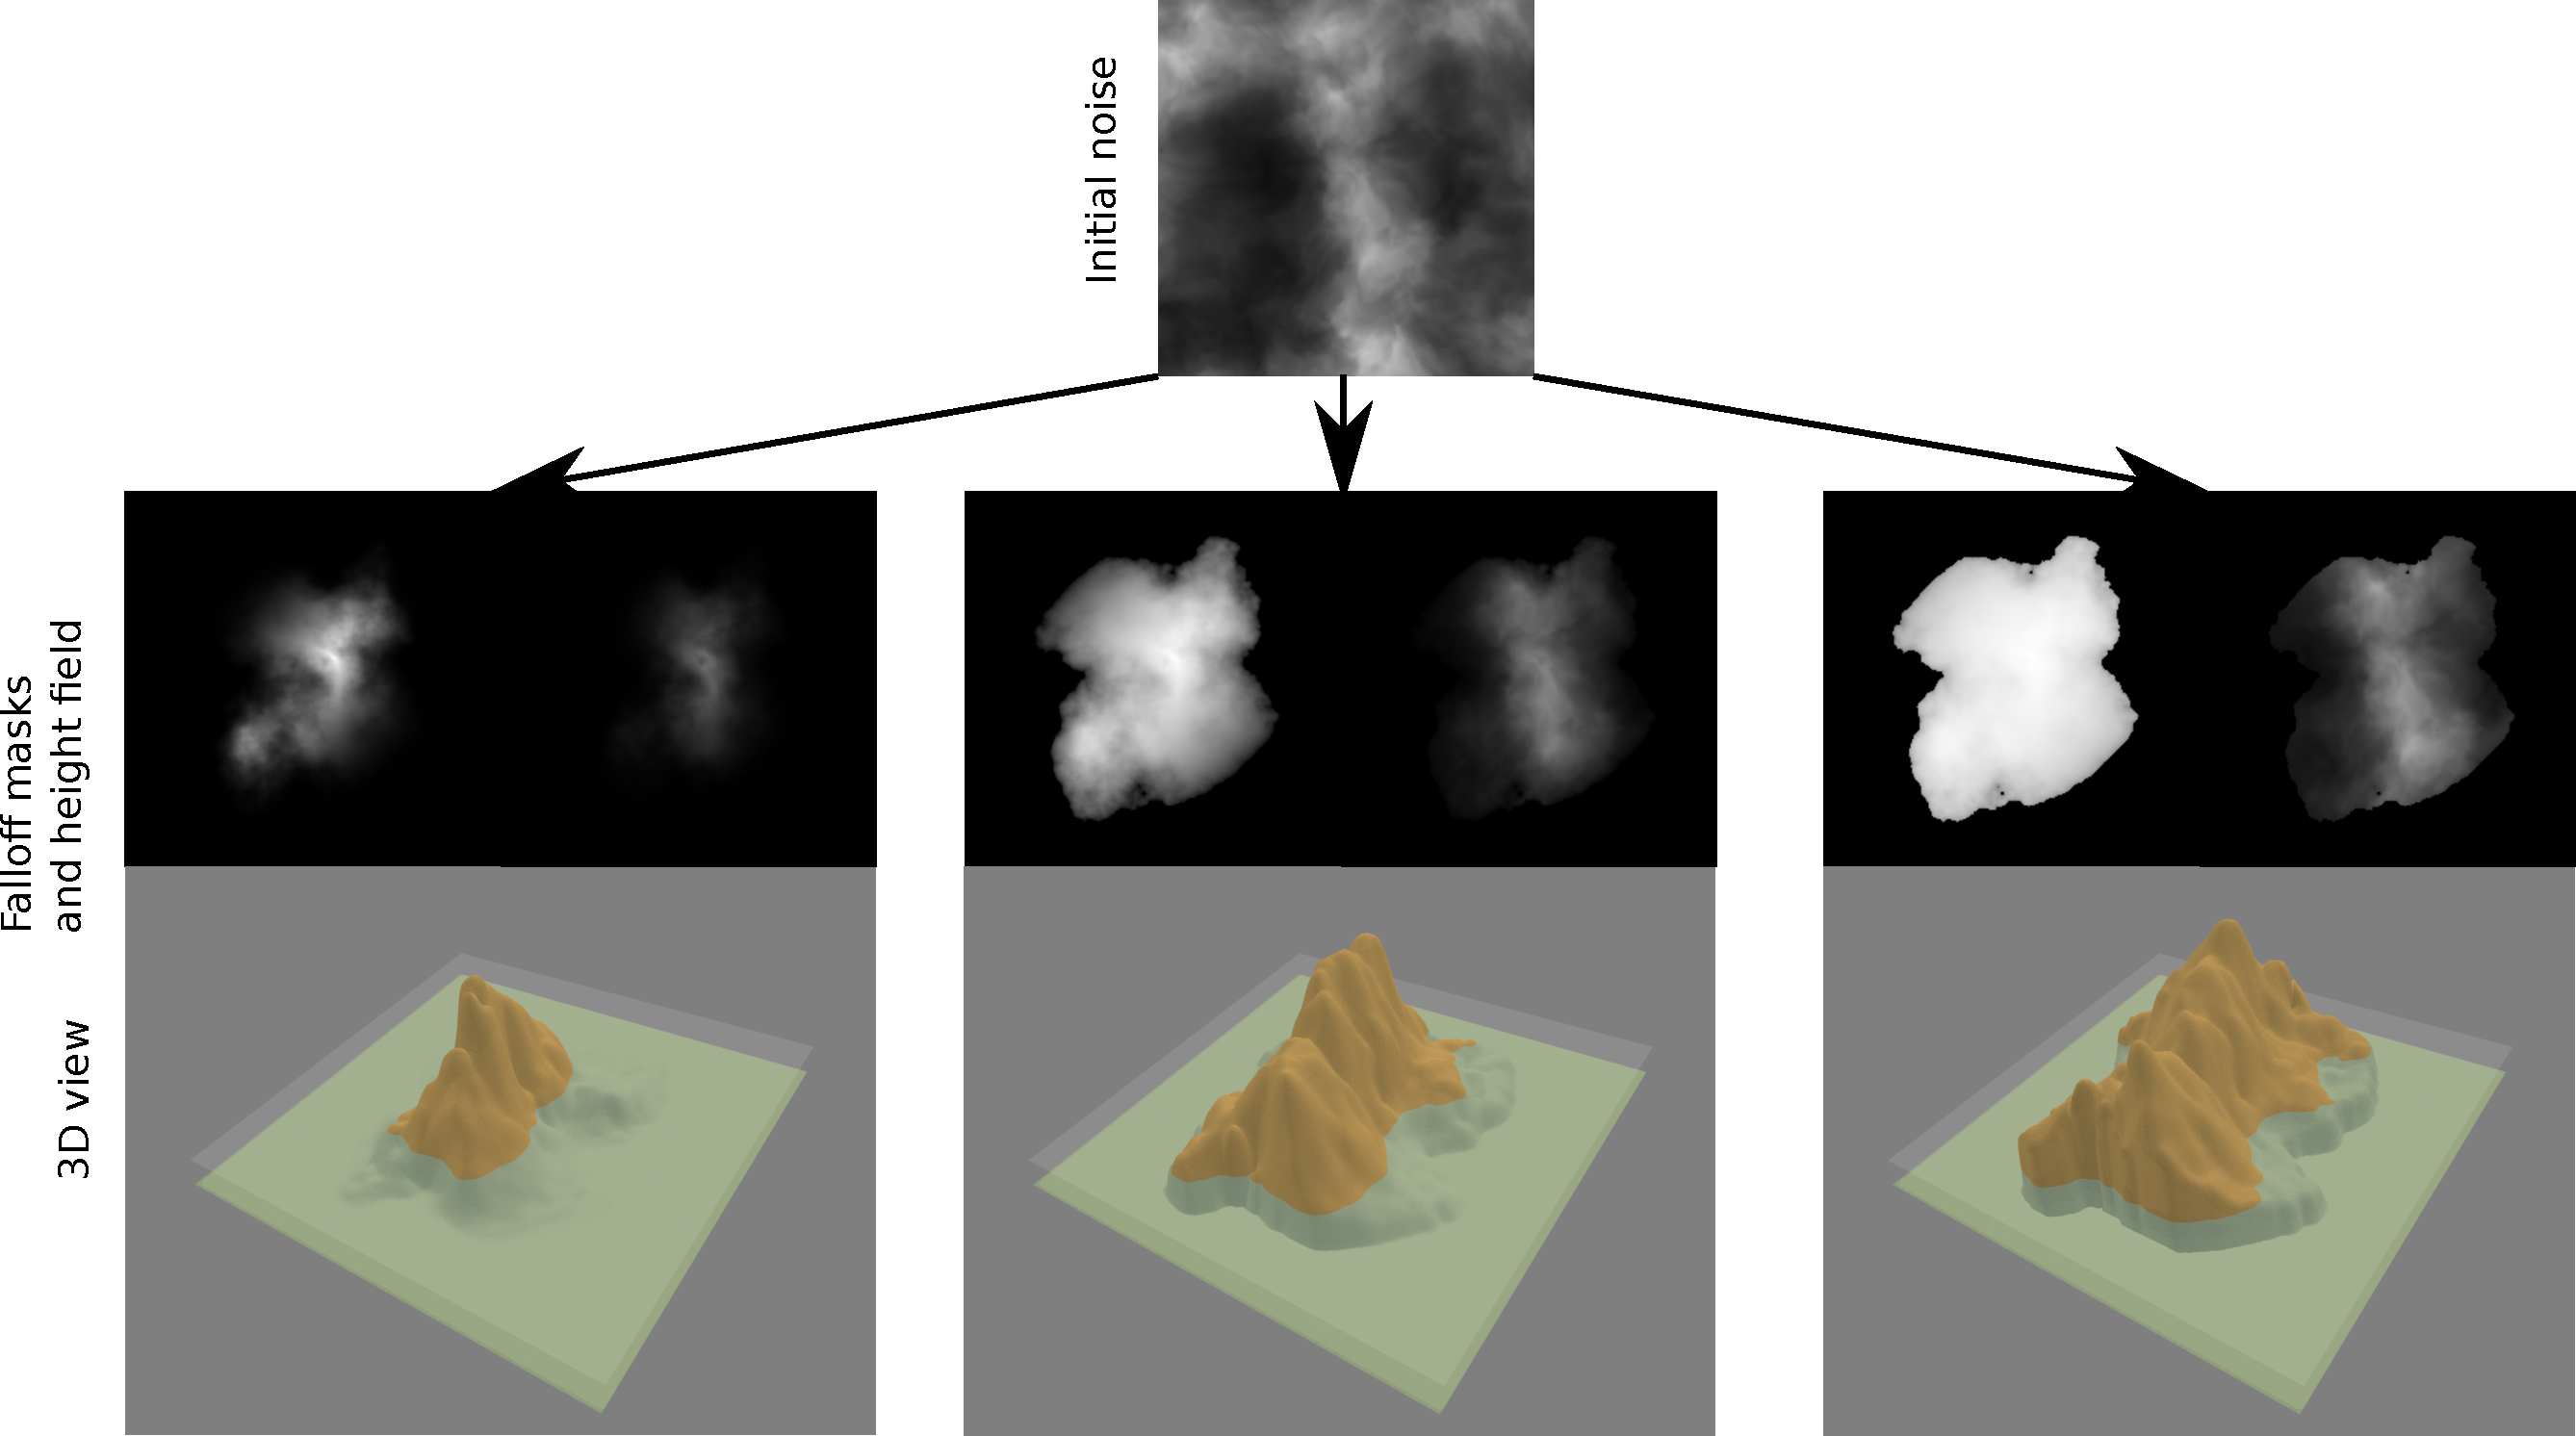
\includegraphics[width = \linewidth]{noise_examples3.pdf}
%     \caption{Three different results of an island generated from noise functions. In each case, the initial height field is the same, computed through flow noise. The falloff masks are also generated with a combination of fBm noise mitigated by the euclidean distance from the image center, warp noise and gamma correction. The only parameter modified for each example is the gamma correction. The results are very different, and hardly controllable. It is also difficult to represent lagoons and reefs using this method.}
%     \label{fig:coral-island_noise-example}
% \end{figure}

% Noise-based procedural generation remains one of the most widely used techniques for creating natural-looking terrains. Perlin noise \cite{Perlin1985}, Simplex noise \cite{Perlin2001}, and the Diamond-square algorithm \cite{Fournier1982} are foundational algorithms that generate pseudo-random yet continuous variations across a grid, producing terrain features that resemble organic landscapes. These techniques have been widely adopted in computer graphics and game development due to their efficiency and visual appeal.

% Beyond basic noise functions, more advanced techniques such as fractal Brownian motion (fBm) and multifractal noise have been introduced to add finer-scale variation and detail \cite{Musgrave1989,Ebert2003}. FBm combines multiple layers, or "octaves," of noise at different frequencies and amplitudes, producing terrains that exhibit more realistic and varied features. The combination of noise with domain warping and signal processing techniques has been explored in depth in procedural modeling literature \cite{Reinhard2010}, enabling further control over visual complexity and terrain realism.

% Noise functions are often paired with falloff maps to produce island-like terrains, where elevation gradually decreases toward the edges of the domain, mimicking coastlines and basic island shapes (see \cref{fig:coral-island_noise-example}). Various methods for enhancing island generation using noise and falloff blending have been proposed for applications in games and virtual worlds \cite{Olsen2004}. While these techniques excel at producing large, visually diverse landscapes quickly, they suffer from several key limitations when applied to the modeling of coral reef islands.

% Critically, noise-based terrains lack grounding in geological or biological reality. They generate spatial patterns through mathematical noise, not through simulations of real-world processes such as volcanic subsidence or coral accretion. The signal processing parameters typically involved (frequency, lacunarity, gain, amplitude, ...) are tuned for visual effect rather than scientific plausibility. As highlighted in procedural modeling surveys \cite{Smelik2009,Galin2019}, this disconnect results in a lack of semantic control and poor correlation with actual environmental dynamics, making it difficult to represent phenomena like reef rings, lagoons, or atoll structures in a biologically or geologically coherent way.

% Moreover, the biological aspects of coral growth are inherently tied to environmental conditions. Coral reefs form and persist only within specific ranges of water depth, sunlight, salinity, and water quality. Their growth patterns are further influenced by ecological health, nutrient availability, and symbiotic relationships. These dependencies are extremely difficult to capture in procedural noise systems, which are not designed to model such complex and coupled dynamics.

% Our approach goes beyond the randomness of noise-based generation by incorporating real-world geological and biological processes into the terrain formation pipeline. Specifically, we model the gradual subsidence of volcanic islands and the upward growth of coral reefs, both of which are central to the long-term evolution of coral reef islands. By embedding these natural processes directly into the generation algorithm, we produce terrains that are not only more realistic but also more controllable. This integration of scientific modeling with procedural flexibility allows us to overcome the inherent limitations of traditional noise-based techniques and more accurately represent the complex formation of coral reef island systems.

% \subsubsection{Simulation-based modeling}

% Simulation-based terrain modeling methods aim to increase realism by replicating natural processes such as erosion, sediment transport, tectonic uplift, and vegetation growth. Unlike noise-based techniques, which rely on random functions, simulation-based approaches model causality and temporal dynamics to describe how a terrain evolves over time under physical or biological forces. These methods are often used to enhance base terrains, adding geologically plausible detail and structure \cite{Benes2006, Smelik2009}.

% \subsubsubsection{Hydraulic and thermal erosion}

% Hydraulic erosion models simulate the impact of flowing water on the landscape by modeling erosion, sediment pickup, transport, and deposition. Early implementations by \cite{Musgrave1989} laid the groundwork for erosion in procedural generation, while more recent works have accelerated these simulations using GPU architectures \cite{Mei2007} and particle-based methods \cite{Neidhold2005}. These simulations often follow Eulerian fluid models or Lagrangian particle systems to capture terrain displacement.

% Thermal erosion, by contrast, simulates mass movement due to gravity, redistributing material from steeper slopes to gentler gradients, akin to landslides or soil creep \cite{Benes2006}. These erosion models generate realistic fluvial networks and landforms, but they are parameter-sensitive and computationally expensive.

% Moreover, such models are generally designed for terrestrial landscapes and lack mechanisms for simulating underwater sedimentation, reef growth, or biogenic processes crucial to coral island formation. These models typically simulate time scales relevant to geomorphological processes (hundreds to thousands of years), which are mismatched with both the faster dynamics of biological processes like coral health and the slower geological evolution of reef islands.

% We will propose our new particle-based erosion simulation method, adapted for underwater and terrestrial landscapes, in \cref{chap:erosion}.

% \subsubsubsection{Tectonic uplift and geologic simulation}

% Geological simulation approaches such as those proposed by \cite{Cordonnier2016, Cordonnier2017a} and extended by \cite{Schott2023} model terrain evolution through crustal deformation and tectonic uplift. These methods simulate isostatic adjustments, plate tectonics, or local uplift phenomena, often over geological timescales.

% Although well-suited for mountain-building processes or fault line modeling, these methods are not designed to account for biogenic terrain formation, such as coral reef accretion, which is critical for simulating coral reef islands. As a result, despite being physically grounded models, they do not capture the coupled geological and biological dynamics necessary for representing the long-term evolution of reef islands.

% \subsubsubsection{Vegetation and ecosystem dynamics}

% Some simulation-based terrain models integrate ecological dynamics to reflect the feedback between terrain and living systems. For instance, \cite{Ecormier-Nocca2021} and \cite{Cordonnier2017b} simulate interactions between vegetation and terrain erosion, modeling plant colonization, growth, and their influence on soil stability and moisture retention.

% These ecosystem simulations allow more complex landscape evolution by considering biotic agents; however, they are designed primarily for terrestrial plants and temperate ecosystems. Coral colonies, in contrast, are marine organisms with strict environmental requirements such as limited depth, adequate sunlight, warm water temperatures, and clear water for photosynthesis via symbiotic algae. Accurately simulating these dependencies would require significant computation resources.

% Furthermore, coral growth is not a passive process like sediment accumulation or root expansion, but an active accretion system that builds calcium carbonate structures over thousands of years. These unique growth mechanisms, constrained by marine ecology, fall outside the scope of existing vegetation or soil-plant-water feedback models.

% \midConclusion

% While simulation-based models represent a significant advancement over purely procedural approaches, they fall short in capturing the coupled geological and biological dynamics that shape coral reef islands. They are either computationally intensive, domain-specific, or biologically inapplicable, highlighting the need for a new class of terrain generation tools that embed long-term marine biogeomorphological processes into the procedural pipeline.




% \subsection{Sketch-based terrain modeling}
% \label{sec:coral-island_sota-sketches}

% The term sketching encompasses several meanings: it can refer to performing gestures with the hand or body, creating a rough drawing, or outlining an idea in a simplified form. Accordingly, sketch-based modeling in 3D computer graphics can be understood through three complementary perspectives, each centered around a distinct core concept.

% First, sketching may focus on interaction, where gestures captured through hand or body motion are used to manipulate virtual objects, often in immersive environments like virtual or augmented reality, drawing on established techniques such as sculpting and distortion \cite{Olsen2009, Cook2009}. Second, it can involve construction, where simple geometric primitives (curves, parametric shapes, implicit surfaces, ...) are combined under constraints to build more complex models. Finally, sketching may center on interpretation, where the user draws strokes on a 2D canvas and the system analyzes their meaning to generate a plausible 3D model.

% While sketch-based modeling encompasses a wide range of techniques, including gesture-driven interaction in immersive environments, this work focuses primarily on the construction and interpretation aspects. In particular, construction serves as the foundation for procedural generation techniques using geometric primitives and constraints (addressed in this section), while interpretation becomes relevant when exploring data-driven approaches using deep learning to infer terrain structure from sketches (discussed in the following section). Interaction-based techniques, though significant in other contexts, fall outside the scope of this work. 

% To distinguish clearly between the different aspects addressed in this chapter, we will refer to the constructive approach as sketch-based, and to the interpretive, learning-driven approach as learning-based. It is important to note, however, that the boundaries between these categories are inherently blurry and often overlap in practice.

% In procedural terrain generation, sketch-based construction approaches enable users to shape landscapes by manipulating high-level geometric primitives through intuitive sketching interfaces. These methods allow the definition of key terrain features, such as mountains, valleys, and coastlines, by drawing their outlines on a two-dimensional canvas, which are then procedurally transformed into 2.5D or 3D terrain representations. This approach offers a high degree of artistic control, making it particularly effective for creative applications like video games and simulations, where modeling is primarily user-driven.

% \subsubsection{Curve-based modeling}

% Sketch-based terrain generation often begins with user-defined curves that act as high-level constraints to guide the shape of the terrain. These curves may represent silhouettes, ridgelines, valleys, or feature outlines. Once defined, they are interpreted by the system and translated into elevation changes through various computational techniques. This approach allows for intuitive control over large-scale landforms while maintaining a procedural foundation for terrain synthesis.

% \AltTextImage{
%     One of the earliest and most influential works in this domain is the system introduced by \cite{Gain2009}, which enables users to sketch silhouettes, ridges, and spine curves to define complex terrain structures (\cref{fig:coral-island_Gain-2009}). The method employs multiresolution surface deformation and propagates wavelet-based noise from the sketched features to their surroundings, allowing users to generate detailed, natural-looking terrains from minimal input. This approach demonstrated the effectiveness of combining intuitive sketch input with procedural detail synthesis.
%     We draw direct inspiration from this work's dual-view sketching strategy, combining top-view and profile sketches, which closely aligns with our concentric curve and height-profile input approach.

%     Expanding on this idea, \cite{Hnaidi2010} proposed a technique based on diffusion equations. In their method, curves are annotated with geometric constraints such as elevation or slope, and a diffusion process is used to interpolate these constraints across the terrain surface. This results in smooth, continuous elevation fields that conform to user-defined features such as rivers, ridgelines, or cliffs. The use of parameterized curves as terrain anchors allows for precise control over landform shaping, while maintaining a high degree of automation.
% }{sketchingGain2009-vertical.png}{caption}{fig:coral-island_Gain-2009}

% \AltTextImage{
%     In a different interaction paradigm, \cite{Tasse2014} introduced a first-person sketching interface, where users draw terrain silhouettes from a particular camera viewpoint (\cref{fig:coral-island_Tasse-2014}). These silhouettes are then projected into 3D, and a deformation algorithm adjusts the terrain so that the drawn features are visible exactly as intended from the user's perspective. This method supports complex silhouettes with occlusions, T-junctions, and cusps, and represents a more immersive and perceptually grounded approach to sketch-based terrain editing.
% }{sketchingTasse2014-vertical.png}{caption}{fig:coral-island_Tasse-2014}

% These methods demonstrate the expressive power of curves as terrain-defining elements. By enabling users to sketch intuitive shapes and constraints, they bridge the gap between artistic intent and procedural complexity. Curve-driven approaches remain foundational in terrain modeling, particularly when user control over large-scale structure is essential. While we do not use the diffusion model, the idea of sketch-defined elevation constraints along curves informs our use of user-defined shape boundaries.


% \subsubsection{Constraint-based modeling}

% While curve-driven techniques provide intuitive shape design, constraint-based and gradient-based approaches focus on exerting precise control over terrain features through formal specifications such as elevation values, slopes, or gradient fields. These methods prioritize structural accuracy and procedural consistency, making them particularly suited to applications that demand terrain realism, integration with geographic data, or fine-grained editing capabilities.

% \AltTextImage{
%     A representative example of constraint-based modeling is presented by \cite{Gasch2020}, who propose a method for procedural terrain generation that respects user-defined elevation constraints (\cref{fig:coral-island_Gasch-2020}). Their system allows users to fix values at specific control points (e.g., paths, landmarks) and then employs a system of equations to propagate these constraints throughout the terrain. Crucially, the method integrates these constraints with a noise-based procedural function to preserve natural randomness while conforming to user intent. This approach is especially valuable when generating terrains that must align with real-world data or gameplay constraints. 
%     We do not adopt their constraint-solving mechanism, but conceptually relate our profile sketch input to a localized height constraint.
% }{sketching-Gasch2020.png}{caption}{fig:coral-island_Gasch-2020}

% \AltTextImage{
%     Extending the idea of constrained procedural generation, \cite{Talgorn2018} introduce a real-time sketch-based terrain generation system based on a GPU-accelerated implementation of midpoint displacement. Users sketch curves with explicit elevation values, which act as absolute constraints, while the system extrapolates and interpolates terrain surfaces in real-time (\cref{fig:coral-island_Talgorn-2018}). Crucially, their model supports both global and local control over interpolation curvature and roughness, and introduces semantic labeling of sketched features (e.g., ridges vs. rivers) to influence how terrain propagates around constraints. This combination of sketch-based input, constraint propagation, and semantic control enables expressive, large-scale terrain modeling at interactive speeds. We do not reuse their fractal interpolation model, but we incorporate their notion of semantic labels and hierarchical constraint propagation to support real-time terrain shaping with sketch-defined features.
% }{sketching-Talgorn2018.png}{caption}{fig:coral-island_Talgorn-2018}

% \AltTextImage{
%     Building on the need for more intuitive editing, \cite{Guerin2022} introduce a novel paradigm by modeling terrain in the gradient domain. Rather than specifying elevation values directly, users interact with slope-based representations, allowing for the manipulation of terrain inclination and the integration of local edits into global terrain structure. By controlling terrain gradients and reconstructing elevation through integration, this method enables seamless blending between regions and supports a more natural editing workflow, particularly for sculpting realistic mountain ridges, valleys, or plateaus (\cref{fig:coral-island_Guerin-2022}). 
%     This gradient-domain editing approach offers interesting insights, but is not directly used, as we operate in the elevation domain with semantic control.
% }{sketching-Guerin2022-vertical.png}{caption}{fig:coral-island_Guerin-2022}

% Both approaches offer complementary strengths: constraint-based methods ensure precise adherence to user-defined features or data sources, while gradient-based systems provide fluid, perceptual control over terrain shaping. Together, they represent a shift toward high-level modeling tools that maintain procedural expressiveness while granting users a deeper degree of terrain control.

% \subsubsection{Semantic terrain representation}
% Beyond geometric sketching and low-level constraints, a third class of methods explores high-level terrain construction, where users guide terrain generation using abstract or semantic inputs. These approaches aim to simplify the authoring process by allowing users to describe what a terrain should contain (e.g., a mountain or a valley) without specifying how to generate it geometrically. Such methods often rely on symbolic sketching, sparse representations, or domain-specific visual cues, offering powerful tools for conceptual design and inverse procedural modeling.

% \AltTextImage{
%     In this vein, \cite{Genevaux2015} propose a method for representing terrains as sparse combinations of procedural primitives, referred to as "terrain atoms." These atoms are stored in a dictionary and can be either extracted from real-world data or generated synthetically. The terrain is modeled as a linear combination of these features, forming a Sparse Construction Tree that blends primitives in a compact and expressive form  (\cref{fig:coral-island_Genevaux-2015}). This representation facilitates terrain editing, amplification, and reconstruction from coarse user input, making it ideal for scenarios that require terrain matching or abstract design control.
%     While this work introduces a symbolic representation of terrain via atoms, it is not reused in our method, which instead relies on semantic label maps. 
% }{sketching-Genevaux2015-1.png,sketching-Genevaux2015-2.png}{caption}{fig:coral-island_Genevaux-2015}

% \AltTextImage{
%     A more illustrative and domain-specific use case is presented by \cite{Natali2012}, who introduce a system for rapid visualization of geological concepts. Here, users sketch schematic representations of subsurface structures such as faults, folds, or strata, and the system generates plausible 3D visualizations of geological terrains. The tool is designed primarily for educational and exploratory purposes, enabling geoscientists and students to create, manipulate, and communicate complex geological scenarios through intuitive sketch input (\cref{fig:coral-island_Natali-2012}). Although it extends beyond traditional terrain elevation modeling, the work exemplifies how sketch-based systems can operate on a conceptual level and support domain-specific semantics.
%     This work inspired our use of sketch strokes to define deformation fields, although our implementation targets structured terrain generation rather than schematic visualization.
% }{sketching-Natali-2012.png}{caption}{fig:coral-island_Natali-2012}

% These high-level approaches demonstrate the potential of sketch-based modeling not just as a geometric tool, but as a semantic interface between human intention and terrain synthesis. By abstracting terrain construction into symbolic or feature-based representations, they allow users to create rich, expressive landscapes without directly engaging with low-level geometry, making them particularly valuable for tasks involving conceptual design, education, and inverse procedural modeling.

% \midConclusion

% The works presented in this section illustrate the diversity of sketch-based approaches for constructive terrain modeling, from curve-driven shape control to constraint-based editing and semantic abstractions. While these methods offer valuable tools for intuitive user interaction and procedural shaping, they often lack ecological grounding, multi-view integration, or the ability to produce structured data suitable for training generative models. In our work, we reinterpret and adapt elements from these approaches such as dual-view sketching, curve-based region definition, and deformation fields, to support the generation of coral reef islands through a hybrid procedural and learning-based pipeline. This constructive sketch-based foundation enables us to balance user control with scalable terrain generation in data-sparse domains.

% % \comment{Also need to include \cite{Ketabchi2016}}


% \subsection{Deep learning}
% \label{sec:coral-island_sota-deep-learning}

% \begin{figure}
% 	\centering
% 	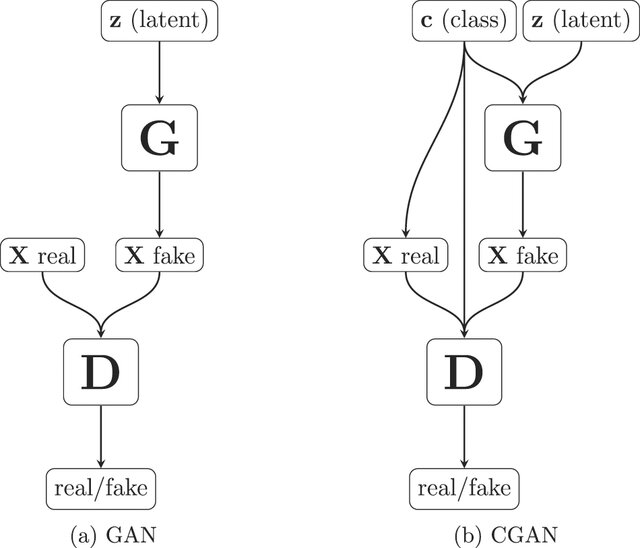
\includegraphics{schemaGAN_cGAN.jpg}
%     \caption{The general structure of GAN and cGAN networks are similar: a generator network $G$ is trained to take some noise $z$ as input to try to create a "realistic" output $X_{fake}$ and a discriminator network $D$ is trained parallelly to distinguish generated data from real data. cGAN networks introduce an information of class $c$ in the input, which is used by the generator and discriminator in their inference process. In the end, only the generator is used to create new data. }
%     \label{fig:coral-island_GAN-scheme}
% \end{figure}

% Over the past decade, deep learning has revolutionized many areas of computer graphics and procedural content creation by learning complex, data-driven priors directly from examples. Unlike purely procedural or sketch-based methods, which rely on hand-tuned noise functions or geometric constraints, neural networks can capture subtle patterns and high-frequency details without explicit programming of each effect. In terrain synthesis, this enables models to infer realistic elevation structures, textures, and region transitions from training data, even when that data is sparse or synthetic. In the context of coral-reef islands where high-resolution digital elevation models are rare, deep learning offers a way to abstract away low-level procedural rules and directly learn the mapping from semantic layouts (label maps) to plausible height fields. In the following sections, we first review general generative adversarial networks (GANs) and then focus on their conditional variant (cGAN), which forms the backbone of our sketch-to-terrain translation pipeline.

% \subsubsection{Generative Aversarial Networks}
% \label{sec:coral-island_sota-GAN}

% Generative Adversarial Networks (GANs), introduced by \cite{Goodfellow2014}, are a class of generative models in which two neural networks are trained in opposition: a generator $G$ learns to produce synthetic data samples that resemble those from a target distribution, while a discriminator $D$ learns to distinguish real samples from those generated. Through this adversarial process, the generator improves its ability to mimic the underlying data distribution, enabling the creation of realistic outputs from random input.

% GANs have been widely adopted for image synthesis, texture generation, and data augmentation, among other tasks. In terrain modeling, they offer the potential to generate plausible landforms by learning directly from real-world data, without requiring hand-crafted procedural rules. The following works demonstrate how different GAN variants have been applied to terrain synthesis, each with its own assumptions, design trade-offs, and limitations.



% Early applications of GANs to terrain focused on unconditional generation, where elevation maps are synthesized from pure latent noise, without any spatial or semantic guidance. \cite{WulffJensen2018} trained a deep convolutional GAN (DCGAN) to produce realistic digital elevation models of mountainous landscapes, showing that terrain-like structures could emerge from purely data-driven learning. The model captured local elevation statistics and allowed for latent space interpolation, enabling smooth variations across generated terrains. However, the lack of spatial conditioning made it difficult to control or constrain specific features such as ridges, valleys, and coastlines, resulting in landscapes that reflected training set distributions but offered no means for intentional design.

% \cite{Spick2019} extended this approach by introducing a Spatial GAN that generates height and texture maps jointly. By conditioning the generation process on spatial coordinates, their model enforced local consistency and reduced structural artifacts. This integration simplified the content pipeline by fusing geometry and appearance into a single pass. Yet despite improved quality, the generation process remained fundamentally uncontrolled: there was no way for users to specify terrain layout, features, or semantics. As with earlier GANs, the model learned to mimic terrain distributions but could not support authoring or guided synthesis.

% To address the lack of control inherent in purely noise-driven GANs, later works introduced multi-stage architectures in which a second, conditional GAN refines or interprets the output of a first-stage generator. \cite{Beckham2017} proposed a two-step pipeline where a DCGAN generates bare terrain heightmaps from noise, and a conditional pix2pix network adds texture based on semantic cues. This separation of geometry and appearance allows for basic stylization and terrain remixing, but still suffers from the lack of control in the initial heightmap generation. In a conceptually similar structure, \cite{Panagiotou2020} reversed the mapping: an unconditional GAN first synthesizes aerial RGB imagery from noise, which is then passed to a cGAN trained to predict plausible DEMs. While this image-to-DEM translation enables realistic terrain reconstruction, it depends on large collections of paired data and lacks any semantic or structural control from the user. In both cases, despite the introduction of a conditional refinement stage, the generation process remains fundamentally anchored in an unconstrained latent input, offering limited authoring capability and no principled way to shape landform structures.

% These approaches show a shift toward using conditional models to guide terrain generation with more structure. But because they still start from random noise, they offer little real control over the layout or meaning of the terrain. A natural next step is to guide the generation process directly from user-defined semantic inputs, such as sketches or label maps, to produce terrain that reflects both the training data and the user's intent.


% \subsubsection{Conditional GANs for terrain generation}
% \label{sec:coral-island_sota-cGAN}

% While traditional GANs generate data from noise, Conditional GANs (cGANs) extend this concept by incorporating side information, often called class map or label map, to guide generation toward user-specified outcomes \cite{Mirza2014}. This makes them particularly attractive for structured content synthesis tasks, including terrain generation, where user input often defines large-scale layout while realism must emerge from learned detail. The pix2pix framework by \cite{Isola2017} is the canonical cGAN formulation for image-to-image translation. It uses a U-Net generator conditioned on an input image (a sketch or a label map, for example), and a PatchGAN discriminator that evaluates realism at the patch level, encouraging fine detail and local consistency.

% \begin{figure}
% \centering
% 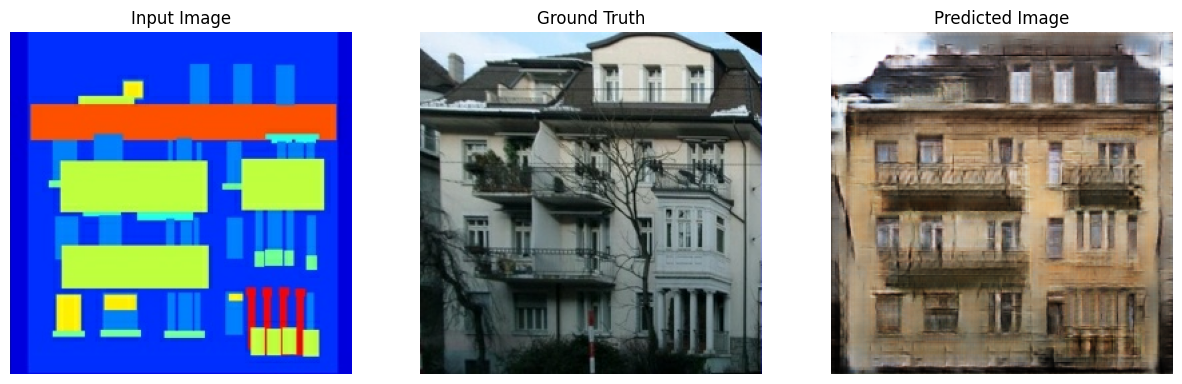
\includegraphics[width = 0.8 \linewidth]{example_pix2pix_facade.png}
% 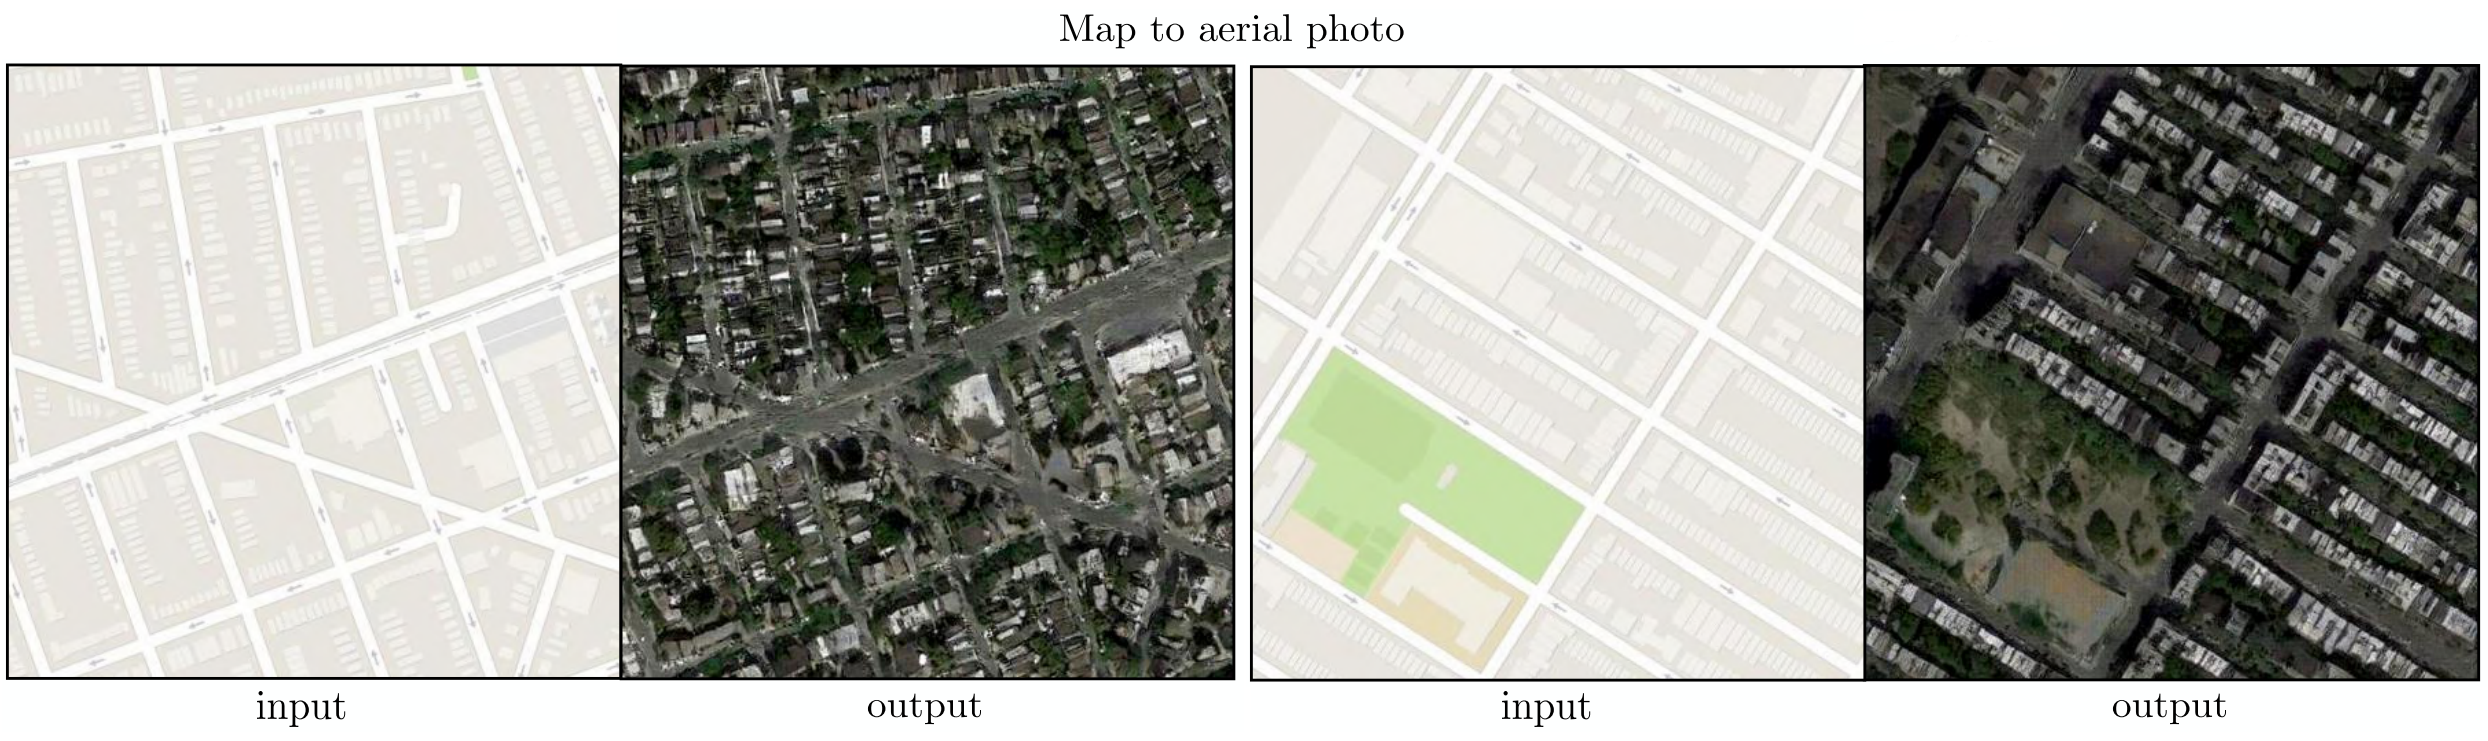
\includegraphics[width = 0.8 \linewidth]{example_pix2pix_maps.png}
% \caption{Example of pix2pix image-to-image translation: (top) a trained model converts semantic label maps into realistic façade images, or (bottom) the construction of highly plausible aerial images from navigation map sketches. This paradigm generalizes to many tasks, including terrain generation.}
% \label{fig:coral-island_pix2pix-example}
% \end{figure}

% In the domain of terrain generation, the use of cGANs remains surprisingly rare. The most directly relevant precedent is the work of \cite{Guerin2017}, who train a pix2pix-style cGAN to map sketched terrain features such as valleys, ridgelines, or peaks, into full-resolution digital elevation models (DEMs). Their results demonstrate that cGANs can plausibly reconstruct complex topographic forms from sparse semantic cues, offering a promising balance between user control and learned realism. Similarly, \cite{Sisodia2022} applies a cGAN to generate stylized terrain heightmaps from sketch maps in the context of 2D game environments, further validating the sketch-to-terrain pipeline.

% Another related line of work explores learning-based terrain synthesis using partial or sparse spatial inputs. \cite{Voulgaris2021} propose a GAN-based system that maps sparse "altitude dot" maps to plausible terrain imagery, acting as a minimal-interaction generative authoring tool. While not strictly a cGAN, their system reflects a similar spirit: conditioning generation on lightweight user constraints. Likewise, \cite{Panagiotou2020} and \cite{Beckham2017} trained a cGAN to invert RGB satellite imagery into elevation data, framing terrain modeling as an appearance-to-geometry and geometry-to-appearance translation task. However, such image-to-DEM (and DEM-to-image) systems are heavily dependent on large paired datasets, which limits their applicability in settings like coral reef islands, where training data are scarce.

% Despite this emerging body of work, there is still no standard pipeline for generating detailed terrains from semantic layout maps using cGANs, particularly in biologically driven environments like coral reef islands. This gap is outstanding given the success of cGANs in analogous image synthesis domains, and the explosive progress in the field of deep generative models. The potential of this approach remains underexploited, especially when it comes to coupling user control with long-term geological plausibility.

% \midConclusion

% In our method, we address this gap by training a pix2pix cGAN to transform label maps (semantic region maps produced by procedural sketch-based modeling) into realistic coral reef island height fields. Each input map encodes key zones of an island (e.g., lagoon, reef crest, beach, island core) using categorical labels, serving as a semantic constraints for terrain synthesis. The cGAN generator learns to condition elevation details on both the global layout and the implicit patterns encoded in the training data. By generating our own synthetic dataset with procedurally modeled coral islands (see \cref{fig:coral-island_difficulties-dataset}), we overcome the shortage of labeled elevation data and enforce geological coherence via data generation design.

% \begin{figure}
% 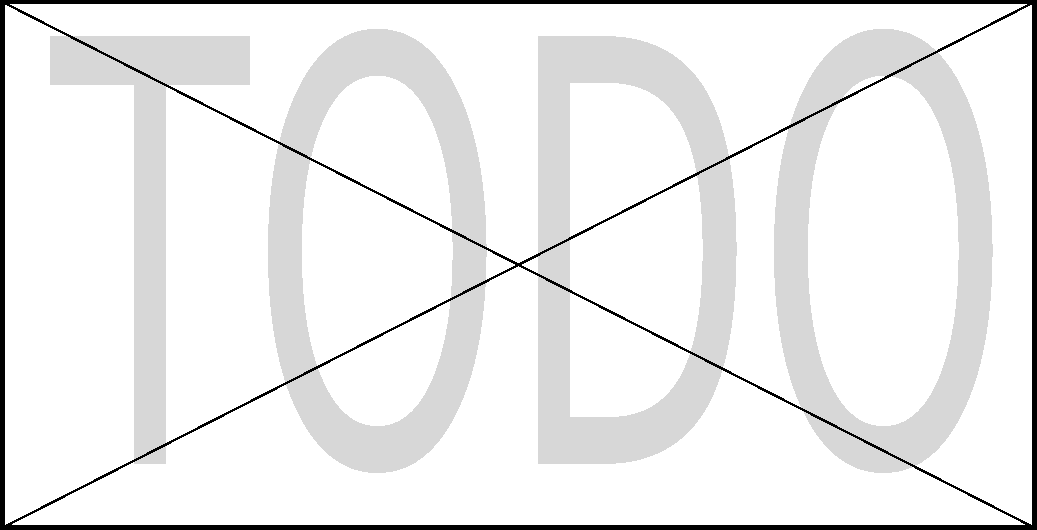
\includegraphics[width=0.9 \linewidth]{placeholder.pdf}
% \caption{Examples of procedural region maps used for training: left to right, canonical island, off-center island, elongated shapes, and multi-island scenes. These maps serve as semantic inputs to the cGAN.}
% \label{fig:coral-island_difficulties-dataset}
% \end{figure}

% This setup offers several key advantages: it respects user-defined structure while allowing the generator to introduce realistic variation, it removes procedural biases such as radial symmetry and fixed island typologies, and it enables the generation of irregular, non-circular landforms while implicitly modeling geological processes like subsidence and coral accretion through training-time priors. 

% In this context, conditional GANs emerge as a powerful yet underutilized tool for terrain modeling. By training on procedurally generated coral island data, we show that sketch-conditioned learning can effectively bridge the gap between high-level user intent and geologically plausible terrain synthesis.
















\section{Overview of our method}


\begin{figure*}[t]
    \includegraphics[]{pipeline_full.pdf}
    \caption{Our method is split in three interleaved stages: the generation process (\cref{sec:coral-island_example-generation}) which creates pairs of height fields and label maps of an island from sketches, the model training (\cref{sec:coral-island_cGAN-training}) which use a synthetic dataset from the previous stage to obtain a cGAN model that generates height fields from label maps to remove the constraints embedded in the initial generation process, and finally, the inference process (\cref{sec:coral-island_results}) uses the trained cGAN to generate the final height fields, including the coral generation process, automatically. }
    \label{fig:coral-island_pipeline}
\end{figure*}

Our method for generating coral reef islands combines user-driven sketching, procedural techniques, and deep learning to create realistic and varied island terrains (\cref{fig:coral-island_pipeline}). 

The pipeline consists of two distinct phases: a procedural data-generation phase and a deep-learning-driven inference phase. 

\subsection{Procedural generation phase}
\label{sec:coral-island_proc-phase}

In the initial procedural phase, the user sketches key island features from two complementary viewpoints: a top view, defining the horizontal layout of island features (island boundaries, beach width, lagoon areas, coral reefs), and a profile view, specifying the vertical elevation profile from island center to ocean (\cref{sec:coral-island_generation-initial}).

Additionally, users can sketch a wind deformation map, enabling simulation of natural erosion patterns caused by wind and waves (\cref{sec:coral-island_wind-deformation}).

From these sketches, the procedural system generates a synthetic island terrain with the keep-up stategy of coral reefs (\cref{sec:coral-island_coral-reef}) and a corresponding semantic label map, where each pixel indicates its region type (island, beach, lagoon, reef, abyss) (\cref{sec:coral-island_procedural-output}).




\subsubsection*{User interaction}
\label{sec:coral-island_description-UI}

\begin{figure}
    \centering
    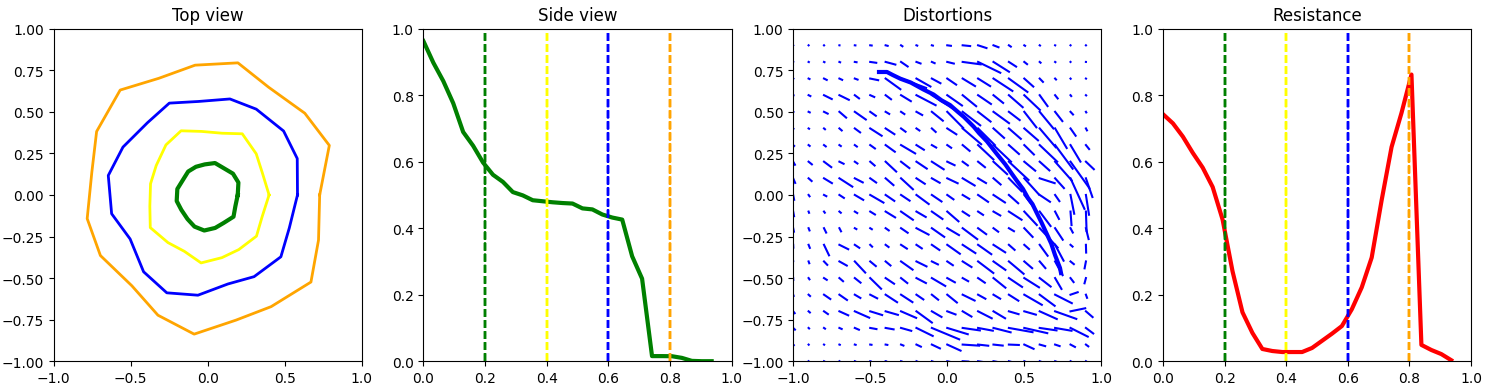
\includegraphics[width = 0.9 \linewidth]{user_interaction_generation.png}
    \caption{The user can interact directly on the island by editing the different canvases in no specific order. This UI shows, from left to right, the top-view sketch with the different outlines of each regions, the profile-view sketch with the outlines represented in dotted lines, the wind velocity sketch drawn with strokes (last stroke is visible), and the resistance function showing here a high resistance at the top of the island and on the front reef.}
    \label{fig:coral-island_wind-from-strokes-interaction}
\end{figure}

As users draw the top-view and profile-view sketches, the system provides real-time feedback on the resulting terrain. The top-view sketch influences the horizontal layout of the island, while the profile-view sketch defines its vertical structure. These sketches can be adjusted independently, allowing the user to fine-tune both the outline and elevation of the island.

While sketching the basic shape, users can apply wind deformation strokes to modify the island's features further. These strokes represent wind and wave influences, distorting the island's shape to introduce more natural, non-radial features such as indentations along the coastline, variable lagoon shapes, or concave formations. The system automatically applies these deformations, providing real-time feedback as the user interacts with the terrain.

This interactive process, combining sketches and wind deformation, allows users to quickly iterate on their designs, refining the terrain to meet specific aesthetic or functional goals.

\subsection{Learning-based generation phase}
\label{sec:coral-island_cGAN-phase}

We repeat this procedural generation process many times with varied parameters (different shapes, scales, subsidence levels, and wind patterns) to create a large synthetic dataset (\cref{sec:coral-island_dataset-generation}). Each dataset entry consists of a label map paired with its procedurally generated terrain height field. Data augmentation is applied to the generated pairs to reduce the impact of the constraints induced from the procedural method (\cref{sec:coral-island_data-augmentation}).

We use this dataset to train a Conditional Generative Adversarial Network (cGAN), specifically the pix2pix architecture, capable of translating label semantic maps into realistic terrain height fields (\cref{sec:coral-island_cGAN-output}).

After training, the procedural step becomes unnecessary. To generate new island terrains, the user only needs to provide a label semantic map as input to the trained cGAN. The cGAN then synthesizes realistic island elevation details directly, capturing learned geological and geomorphological patterns from the synthetic training data (\cref{sec:coral-island_results}).

\subsubsection*{User interaction}
\label{sec:coral-island_cGAN-phase-interaction}

Thus, the trained cGAN provides a user-friendly interface: users draw or edit simple label maps (regions) to rapidly generate diverse, geologically plausible coral reef island terrains, incorporating realistic features such as smooth transitions between regions, detailed coral reef structures, and naturally varied shapes free from procedural constraints.

\midConclusion

This combined procedural-and-learning approach provides a simple, flexible, and powerful tool for island terrain generation, enabling users to intuitively generate realistic and diverse coral reef islands aligned with real-world geological and biological processes such as volcanic subsidence, coral reef growth, and wind-driven erosion.
















\section{Procedural terrain generation}
\label{sec:coral-island_example-generation}

% \begin{figure}
% 	\centering
% 	\autofitgraphics[]{placeholder.pdf}
%     \caption{The example generation fully takes its potential in the procedural techniques, using sketches from the user (top-view sketch, profile-view sketch, wind sketch, and resistance sketch) to generate a height field in accordance with a label map. }
%     \label{fig:coral-island_example-pipeline}
% \end{figure}

The generation of coral reef island terrains involves a structured process that takes the user's sketches and produces a complete 3D terrain model. This process begins with the creation of the initial height field based on the user's input, followed by the application of wind deformation to introduce natural variations, and concludes with the integration of coral reef features through subsidence and coral growth modeling.




The generation of coral reef islands in this system begins with two intuitive sketch-based inputs from the user: a top-view sketch and a profile-view sketch, which define the islands horizontal layout and vertical elevation profile. In addition to these sketches, the user can further refine the terrain by applying wind deformation strokes, which simulate the effects of wind and waves on the islands shape. This combination of sketches and wind inputs gives users precise control over both the islands structure and its natural variations, such as irregular coastlines or concave features. We will present the usefulness of these sketches in this section, and describe the technical details in the next section.



\subsection{Initial height field generation}
\label{sec:coral-island_generation-initial}


% % \begin{figure}
% % 	\centering
% %     \autofitgraphics[]{Cicia_island.png, Cicia_island-outlines.png}
% % 	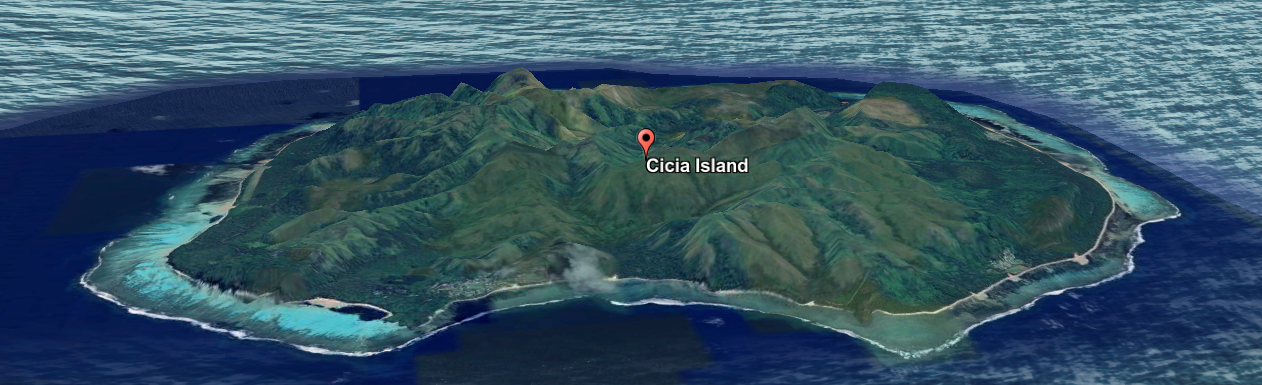
\includegraphics[width=0.90 \linewidth]{Cicia_island-3D.png}
% %     \caption{(Left) A real world example of aerial image (and 3D visualization on bottom) of an island (Cicia Island) may be segmented in regions. (Right) We can represent the different regions by the boundaries they form.}
% %     \label{fig:coral-island_top-view-sketch}
% % \end{figure}

% The top-view sketch defines the islands outline as seen from above. Using a simple drawing interface, the user can delineate the boundaries between key regions of the island, including the island itself, the beaches, the lagoon, and the surrounding abyss. The system assumes that these regions are arranged concentrically around the center of the island, with each boundary defined by a radial distance from the center.

% Each region's boundary is represented in polar coordinates, with $\radius_\p$ indicating the radial distance from the islands center and $\angl_\p$ representing the angular position. This polar representation allows the system to map the users sketch onto a circular framework, ensuring smooth transitions between regions and maintaining a coherent layout for the island.

% In this sketch, the user defines the overall horizontal layout of the island, including the size and shape of each feature. Variations in the outline are introduced by allowing the radial distances to vary with angle, ensuring that the island is not strictly symmetrical and introducing more natural, irregular shapes.

% \begin{figure}
%     \autofitgraphics[]{binary-heights-input-only-outlines-2.png, binary-heights-output-only-heightmap-2.png, binary-heights-render-2.png}
%     \caption{Using only the outlines of the island as a input sketch, we can provide a height to each point of the field depending on the region in which it rely.}
%     \label{fig:coral-island_procedural-height-only}
% \end{figure}



% % \begin{figure}
% % 	\centering
% %     \autofitgraphics[]{profileFunction.pdf, schema_profile.jpg}
% %     \caption{(Left) A profile function $\heightProfile$ is defined as a 1D function and represents the surface from the center of the island to the abysses. (Right) The cross-section representation of an island is often represented as a 1D function defined using terrain features as landmarks. }
% %     \label{fig:coral-island_profile-function}
% % \end{figure}

% The profile-view sketch defines the vertical elevation profile of the island along any radial direction, offering control over the islands height. In this view, the user specifies the elevation of different regions of the island, such as the island peak, beach, lagoon, abyss, and everything in-between, by drawing the corresponding profile curve.

% The regions outlines correspond to key terrain transitions: the highest point of the island (center), the island border, the beach, the lagoon, and the deep-sea abyss. The system uses these milestones to interpolate a continuous 1D height function $\heightProfile(\distRegions)$, where $\distRegions$ represents a non-uniform region distance from the islands center, and $h = \heightProfile(\distRegions)$ gives the height at each point. This continuous profile ensures smooth elevation transitions across the island.

% By combining the top-view and profile-view sketches, the system can generate a full 3D terrain model that accurately reflects the users design by revolution modeling.

% The generation of the coral reef island terrain begins by transforming the user-defined top-view and profile-view sketches into a coherent 3D height field. This process combines the radial layout of the top-view sketch with the elevation information provided by the profile-view sketch, creating a terrain that accurately represents the desired features, such as the island, beaches, lagoons, and abyss.

% For any point $\p$ on the terrain, the system first computes the polar coordinates $(\radius_\p, \angl_\p)$, where $\radius_\p$ is the radial distance from the island's center, and $\angl_\p$ is the angular component. The radial distance $\radius_\p$ is used to determine which region the point belongs to (island, beach, lagoon, reef, or abyss). The user-defined outlines in the profile sketch specify the radial limits between these regions.

% % \AltTextImage{
%     % Each point's height is determined by the profile function $\heightProfile(\distRegions)$, where $\distRegions$ represents a "piecewise parametric distance" from the island's center. The piecewise parametric distance works by dividing the radial distance from the center into segments, defined by these region boundaries. Each segment corresponds to a distinct region of the terrain, and within each segment, the distance $\distRegions$ is interpolated between the region boundaries. For a point $\p$ lying between two boundaries $\Radius_{i}$ and $\Radius_{i+1}$, the distance $\distRegions_\p$ is calculated as:

%     % \begin{align}
%     %     \distRegions_\p = i + \frac{\radius_\p - \Radius_{i}}{\Radius_{i + 1} - \Radius_{i}}
%     % \end{align}
%     % where $i$ is the index of the nearest lower region boundary. This method allows for smooth transitions between regions, even when the spacing between boundaries varies. 

%     % For any point $\p$, the height is finally computed as:
%     % \begin{align}
%     %     h(\p) = \heightProfile(\distRegions_\p)
%     % \end{align}
% % }{outlines-top-view-x-bar.pdf, outlines-result-x-bar.pdf}{The $\tilde{x}$ parameter is used to stretch the 1D height function $\heightProfile(x)$ to fit the distances from the center to the outlines of each region defined in the top-view sketch.}{fig:coral-island_parametric-distance}
% \wrapFig{outlines-top-view-x-bar.pdf}{.3}{label}{caption}

% Each point's height is determined by the profile function $\heightProfile(\distRegions)$, where $\distRegions$ represents a parametric region distance from the island's center. 

% Instead of using the raw radial distance $\radius_\p$, we define $\distRegions_\p$ to map each point to a normalized position along the sequence of terrain regions. The radial space is divided by the user-defined boundaries $\Radius_0, \Radius_1, ..., \Radius_n$ corresponding to the island, beach, lagoon, and abyss.

% For a point $\p$ lying between two boundaries $\Radius_{i}$ and $\Radius_{i+1}$, its parametric distance is defined as:

% \begin{align}
%     \distRegions_\p = i + \frac{\radius_\p - \Radius_{i}}{\Radius_{i + 1} - \Radius_{i}}
% \end{align}

% Here, $i$ is the index of the region containing $\p$ ($\Radius_i \leq \radius_\p < \Radius_{i+1}$). This formula maps the region's radial span to the interval $[i, i+1]$, ensuring smooth and consistent interpolation between adjacent regions.

% The final height at point $\p$ is computed by evaluating the elevation profile:
% \begin{align}
%     h(\p) = \heightProfile(\distRegions_\p)
% \end{align}
The top-view sketch defines the island's outline as seen from above. Using a simple drawing interface, the user delineates concentric boundaries for key regions such as the island itself, the beaches, the lagoon, and the surrounding abyss, around the canvas center. Each boundary is represented in polar coordinates, where $\radius_\p$ is the radial distance from the island's center and $\angl_\p$ is the angular position. Allowing $\radius$ to vary with $\angl$ introduces irregular, natural shapes rather than perfect circles (\cref{fig:coral-island_procedural-height-only}).

\begin{figure}
    \autofitgraphics[]{binary-heights-input-only-outlines-2.png, binary-heights-output-only-heightmap-2.png, binary-heights-render-2.png}
    \caption{Using only the outlines from the top-view sketch, each point in the field is assigned a region (island, beach, lagoon, abyss), which later guides its height assignment.}
    \label{fig:coral-island_procedural-height-only}
\end{figure}

The profile-view sketch defines the island's vertical elevation along any radial direction. Here, the user draws a curve that specifies height at key terrain milestones, such as the central peak, island border, beach, lagoon, and abyss, creating a continuous 1D height function $\heightProfile(\distRegions)$ where $\distRegions$ is a parametric distance measuring position along the sequence of regions. This continuous profile ensures smooth elevation transitions across all terrain features.

\wrapFigR{outlines-x-bar.pdf}{.3}{fig:coral-island_parametric-distance}{Parametric distance $\tilde x$ depending on angle $\angl$. } %{The 3D terrain is generated by revolving the 1D height function $h(\tilde{x})$ around the center of the island. The colored base (green, yellow, blue) represents user-defined regions from the top-view sketch. The dark green surface corresponds to the elevation profile $h(\tilde{x})$, sampled along radial directions. Vertical slices show how each angle uses the same elevation curve.}

By combining the top-view and profile-view sketches via revolution modeling, the system generates a full 3D terrain model that matches the user's design. The process begins by transforming those two sketches into a coherent height field (\cref{fig:coral-island_procedural-smooth-heights}).

For any point $\p$ on the terrain, the system computes polar coordinates $(\radius_\p, \angl_\p)$. The radial distance $\radius_\p$ determines which region the point belongs to (island, beach, lagoon, reef, or abyss) based on the user-defined radial limits. Those outlines from the top-view sketch provide the exact boundaries between regions.

Each point's height is computed using the profile function $\heightProfile(\distRegions)$. Instead of using the raw radial distance $\radius_\p$, we define a parametric region distance $\distRegions_\p$ that maps each point to a normalized position along the concentric regions (see \cref{fig:coral-island_parametric-distance}). The radial space is divided by user-defined boundaries $\Radius_0, \Radius_1, \dots, \Radius_n$, corresponding to the island center, border, beach, lagoon, and abyss.


When a point $\p$ lies between two boundaries, say $\Radius_{i}$ and $\Radius_{i+1}$, its parametric distance is
\begin{align}
    \distRegions_\p = i \;+\; \frac{\radius_\p - \Radius_{i}}{\Radius_{i + 1} - \Radius_{i}},
\end{align}
where $i$ is the index of the region containing $\p$ (i.e., $\Radius_i \le \radius_\p < \Radius_{i+1}$). This linear mapping stretches each region's radial span to the interval $[i,\,i+1]$, ensuring smooth interpolation across region boundaries. The final height at point $\p$ is then
\begin{align}
    h(\p) = \heightProfile(\distRegions_\p).
\end{align}

\begin{figure}
    \autofitgraphics[]{smooth-input-outline-heights-1.png, smooth-output-heights-1.png, smooth-render-1.png}
    \caption{Given top-view and side-view outlines, the 3D result is be obtain by revolution. }
    \label{fig:coral-island_procedural-smooth-heights}
\end{figure}

% This approach ensures that the height field accurately follows the elevation profile specified by the user while maintaining smooth transitions between different regions of the island.

% The result is a height field that captures both the radial structure of the island (from the top-view sketch) and the vertical elevation profile (from the profile-view sketch), producing a realistic representation of islands with smooth transitions between the key terrain features.

\begin{deferredfigure}
    \autofitgraphics[]{smooth-input-outline-heights-1.png, smooth-output-heights-1.png, smooth-render-1.png}
    \autofitgraphics[]{smooth-input-outline-heights-2.png, smooth-output-heights-2.png, smooth-render-2.png}
    \autofitgraphics[]{smooth-input-outline-heights-3.png, smooth-output-heights-3.png, smooth-render-3.png}
    \caption{Providing a smooth function between each region results in islands with plausible reliefs. We fixed the outlines while editing only the height function in order to produce, from top to bottom, a low island, a coral reef island, and finally an identical island without the reef. }
    \label{fig:coral-island_procedural-smooth-heights-multiple-examples}
\end{deferredfigure}





\subsubsection{Wind deformation}
\label{sec:coral-island_wind-deformation}

% % \begin{figure}
% %     \centering
% %     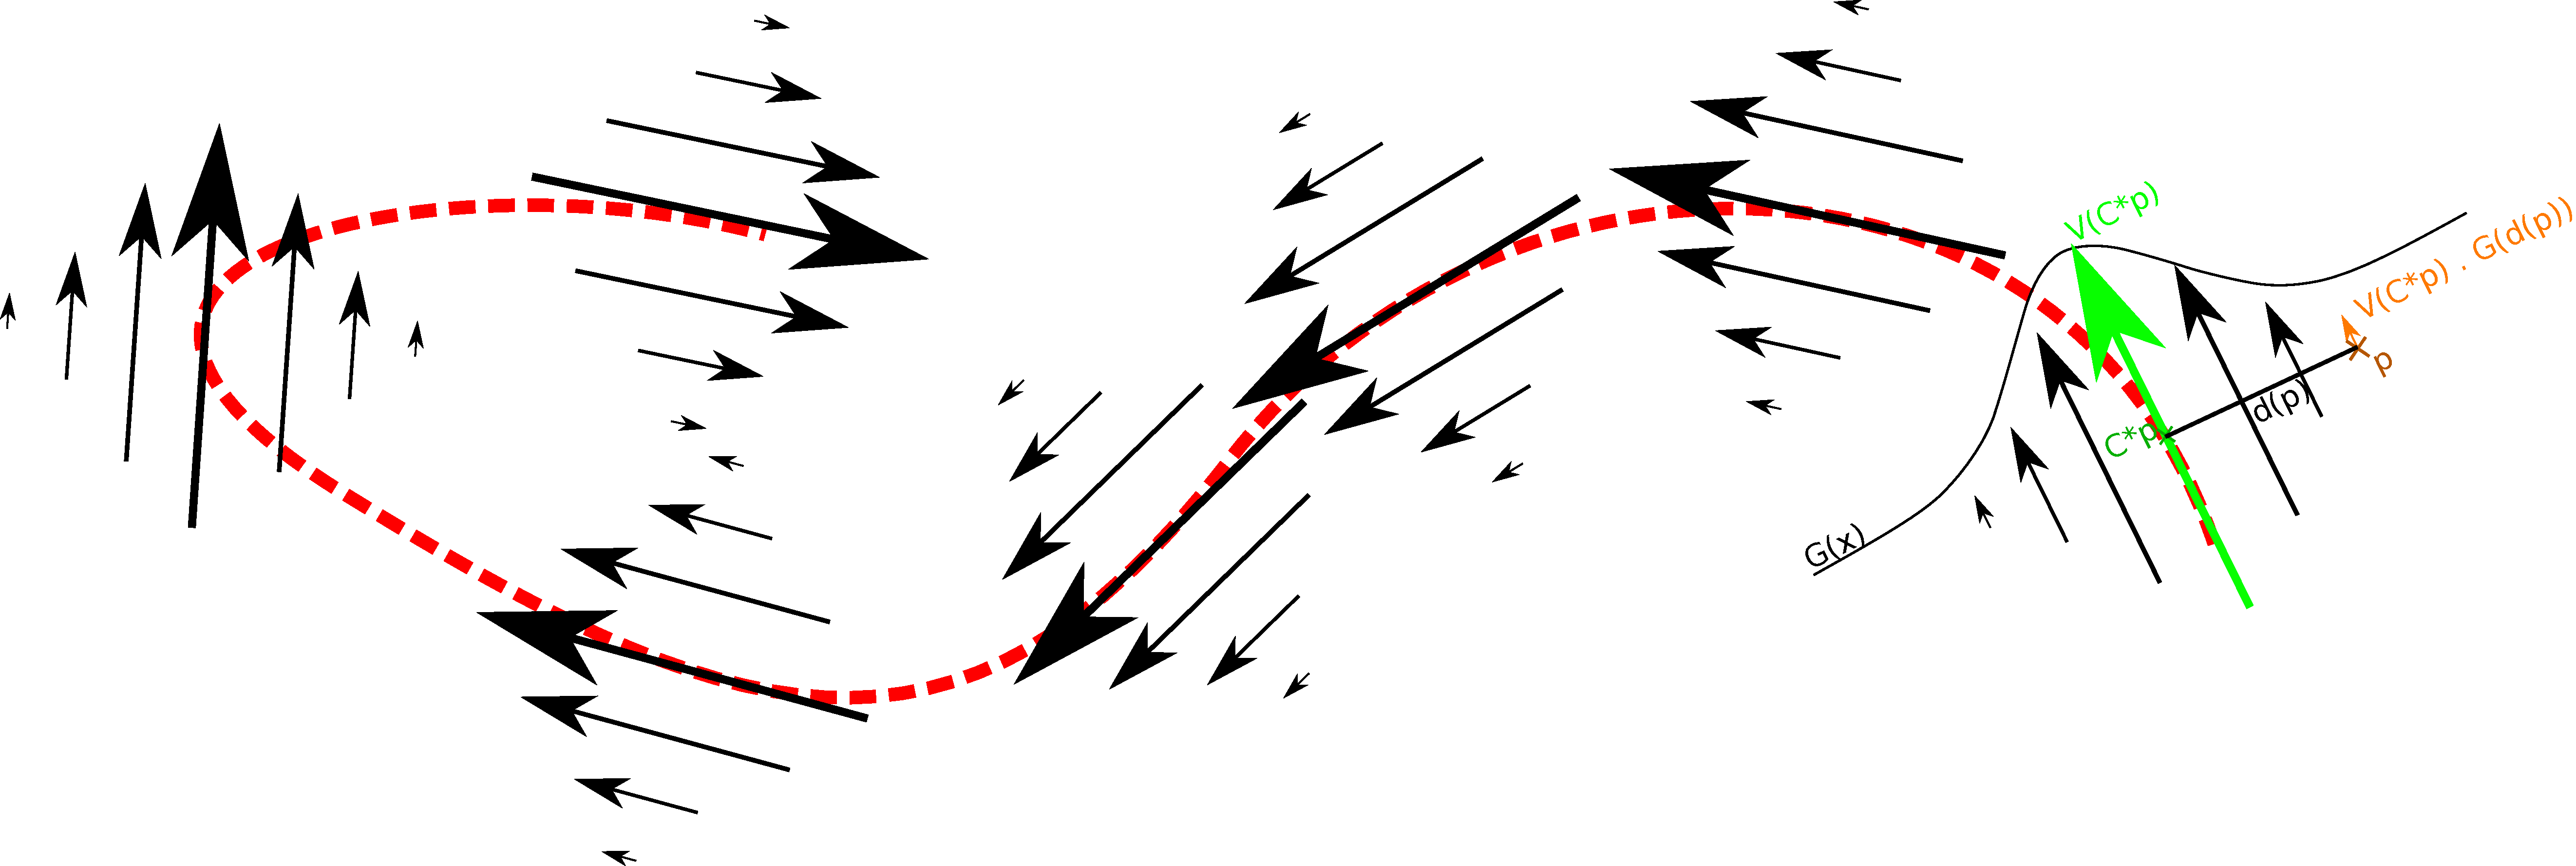
\includegraphics[width = 0.8 \linewidth]{windByStrokes.pdf}
% %     \caption{From the parametric curve defined by a user (red), we define the velocity field by considering the velocity (first derivative) of the curve at the closest point $\closestCp$, modulated by a gaussian distance function $G(x)$. }
% %     \label{fig:coral-island_wind-from-strokes}
% % \end{figure}

% In addition to the sketches, the user can influence the shape of the island by defining a wind velocity field. This field simulates the effects of wind and wave erosion on the island's surface, introducing natural deformations such as coastline indentations, and more importantly allow the user to break the radial symmetry constraint.

% The wind field is represented as a series of wind strokes drawn by the user on a 2D canvas. Each stroke represents a parametric curve, where the direction and strength of the wind are encoded as a vector field. The user controls the wind's direction by drawing these curves, and the system interprets the strokes to create a velocity field that defines how the terrain should be deformed.

% As the user draws a wind stroke, the system generates a set of control points along the curve, with the option to adjust the stroke's width. The width of each stroke determines the area of influence around the curve, where wider strokes result in broader deformations of the terrain.
% The deformation strength decreases with distance from the wind curve using a Gaussian falloff function using the stroke width as standard deviation, ensuring that the terrain transitions smoothly from deformed regions to non-deformed areas.
% Once the wind strokes are applied, the system processes the wind velocity field by displacing the terrain points accordingly. The height field, originally generated from the user's sketches, is modified by the wind field to create non-radial features, breaking the initial radial symmetry and producing a more organic island shape.

% After generating the initial height field based on the top-view and profile-view sketches, the next step in the process introduces wind deformation. This step simulates the long-term effects of wind and wave erosion, breaking the radial symmetry of the terrain and adding natural variations such as concave coastlines and irregular island shapes.

% The wind deformation can be controlled through a user-defined vector field, which represents the direction and strength of wind flows across the terrain. Users interact with the system by drawing strokes on a 2D canvas, which are then interpreted as parametric curves $\curve$ representing wind patterns. Each stroke defines a wind flow in the curve's direction $\curve'$, a strength $S$, and an effect width $\std$; these wind flows are used to displace the terrain, simulating the gradual reshaping of the island due to wind and wave erosion.

% The strokes are represented as Catmull-Rom splines, a type of parametric curve that allows for smooth, continuous wind paths. For any point $\p$ on the terrain, the deformation vector $\warp(\p)$ is calculated based on the proximity of $\p$ to the nearest wind strokes. The strength of the displacement is controlled by a Gaussian scaling function, which ensures that points closer to the wind strokes experience stronger displacement, while points farther away are less affected.

% The displacement function $\warp(\p)$ is computed as a sum of the influences from all nearby wind strokes. For each stroke, the deformation vector is scaled by a Gaussian function that smoothly decreases with the distance from $\closestCp$ the closest point on the parametric curve $\curve$, as follows:

% \begin{align}
%     \warp(\p) = \sum_{\curve \in \text{curves}} S \frac{\curve'(\q)}{\| \curve'(\q) \| } \cdot G_\std\left(\| \p - \closestCp \| \right)\\
%     G_\std(x) = \frac{1}{\std \sqrt{2\pi}} e^{-\frac{x^2}{2 \std^2}}
% \end{align}

% Once the deformation vector $\warp(\p)$ is computed, the terrain height at point $\p$ is adjusted by displacing $\p$ to a new point $\warp(\p)$.
% We can then compute the final height $h(\warp \circ \p) = \heightProfile(t_{\p})$, or, as the implicit modeling community would write it, 
% \begin{align}
%     \Tilde{h} = \warp^{-1} \circ h
% \end{align}

% This process introduces variations in the terrain, distorting the coastline, creating concave regions, and breaking the original radial symmetry defined by the top-view and profile-view sketches.


% To ensure that certain regions of the terrain, such as deep-water areas, remain relatively unaffected by the wind, a resistance function $\resistance(\distRegions)$ is applied. The resistance function modulates the effect of the wind deformation based on the previously computed piecewise parametric distance $\distRegions$, with the same interaction means than the $\heightProfile$ function.

% The resistance function $\resistance(\distRegions)$ is defined similarly to the profile function, and it controls the magnitude of the displacement at each point. For example, regions near the coastline (such as the beach and lagoon) might have lower resistance, allowing for more significant deformation (simulating coastal erosion from wave-energy), while regions farther away (such as the abyss) have higher resistance, limiting the wind and coastal erosion impact.

% The deformation vector previously described is scaled by the resistance function at each point $\p$, such that the final deformation vector becomes:

% \begin{align}
%     \Tilde{\warp}(\p) = \left(1 - \resistance(\distRegions_\p) \right) \cdot \warp(\p)
% \end{align}

% This ensures that the wind deformation has the greatest impact on areas like the coastline and beach, where erosion naturally plays a larger role, while deeper regions like the abyss or stronger regions like mountains remain stable and relatively unchanged.

% \begin{deferredfigure}
%     \autofitgraphics[]{result_low_resistance.png, result_high_resistance.png}
%     \caption{(Left) Given a uniform wind velocity field and a resistance function similar as \cref{fig:coral-island_resistance-function}, the coasts are smoothly eroded while the interior of the island is almost unaffected. (Right) Modifying the resistance function to affect a strong resistance to borders simulate the effect of coast reinforcements.}
% \end{deferredfigure}

% The wind deformation process results in a modified height field where the terrain has been warped according to the user-defined wind strokes. This deformation introduces non-radial features, such as concave coastlines or irregularities along the beach and lagoon, making the island appear more natural and varied.

% Both the height field and the label map (which tracks the terrain regions) are updated to reflect the wind deformation. This ensures that the semantic information of the terrain remains consistent even after the terrain has been warped. The label map is deformed in the same way as the height field, preserving the logical structure of the island for further post-processing, such as texturing.

% For instance, consider a simple circular island generated from the initial height field. By applying wind strokes along one side of the island, the deformation process can create concave regions along the coastline, making the shape more irregular and mimicking the effects of real-world wind and wave erosion. The resistance function ensures that while the beach and lagoon areas are deformed, the abyss remains largely unaffected as they are far from the wind and wave effective areas, preserving the island's overall structure.

\begin{figure}
    \autofitgraphics[]{wind-deform-input.png}
    \autofitgraphics[]{wind-deform-output-original.png, wind-deform-render-original.png, wind-deform-output.png, wind-deform-render.png}
    \caption{Defining a top-view wind vector field from user-provided strokes (top, blue) in association with a resistance function (top, red), a height field is deformed accordingly. Right: original height field and render; Left: altered results. The beach and lagoon regions are defined with low resistance, which is visible by having only these resgions deformed in bottom results. }
    \label{fig:coral-island_wind-effect-result}
\end{figure}

To break the radial symmetry inherent in sketch-based terrain generation and introduce more organic island shapes, we allow the user to define a wind velocity field via freehand strokes on a 2D canvas. Each stroke is represented as a parametric curve $\curve$, interpreted as a local wind flow with direction $\curve'$, strength $S$, and influence width $\std$. These strokes simulate wind and wave erosion effects on the terrain.

The deformation vector at any terrain point $\p$ is computed as a sum over all strokes, weighted by a Gaussian falloff centered on the closest point $\closestCp$ along each curve (\cref{fig:coral-island_wind-effect-result}, top):

\begin{align}
    \warp(\p) = \sum_{\curve \in \text{curves}} S \frac{\curve'(\q)}{\| \curve'(\q) \| } \cdot G_\std\left(\| \p - \closestCp \| \right), \quad
    G_\std(x) = \frac{1}{\std \sqrt{2\pi}} e^{-\frac{x^2}{2 \std^2}}.
\end{align}

To preserve semantic structure across terrain regions, a resistance function $\resistance(\distRegions)$ modulates the deformation based on terrain zones such as beach, lagoon, or abyss (\cref{fig:coral-island_resistance-result}). The final deformation vector becomes:

\begin{align}
    \Tilde{\warp}(\p) = \left(1 - \resistance(\distRegions_\p) \right) \cdot \warp(\p).
\end{align}

This warp is applied to both the height field and the label map, ensuring consistent semantic deformation. For example, applying strokes to one side of a circular island creates concave coastlines while leaving high-resistance regions (e.g., the abyss) unaffected, simulating the localized impact of natural erosion (\cref{fig:coral-island_wind-effect-result}, bottom).

\begin{figure}
    \autofitgraphics[]{result_low_resistance.png, result_high_resistance.png}
    \caption{(Left) Given a uniform wind velocity field and a resistance function similar as \cref{fig:coral-island_resistance-function}, the coasts are smoothly eroded while the interior of the island is almost unaffected. (Right) Modifying the resistance function to affect a strong resistance to borders simulate the effect of coast reinforcements.}
    \label{fig:coral-island_resistance-result}
\end{figure}

% \begin{figure}
% 	\centering
% 	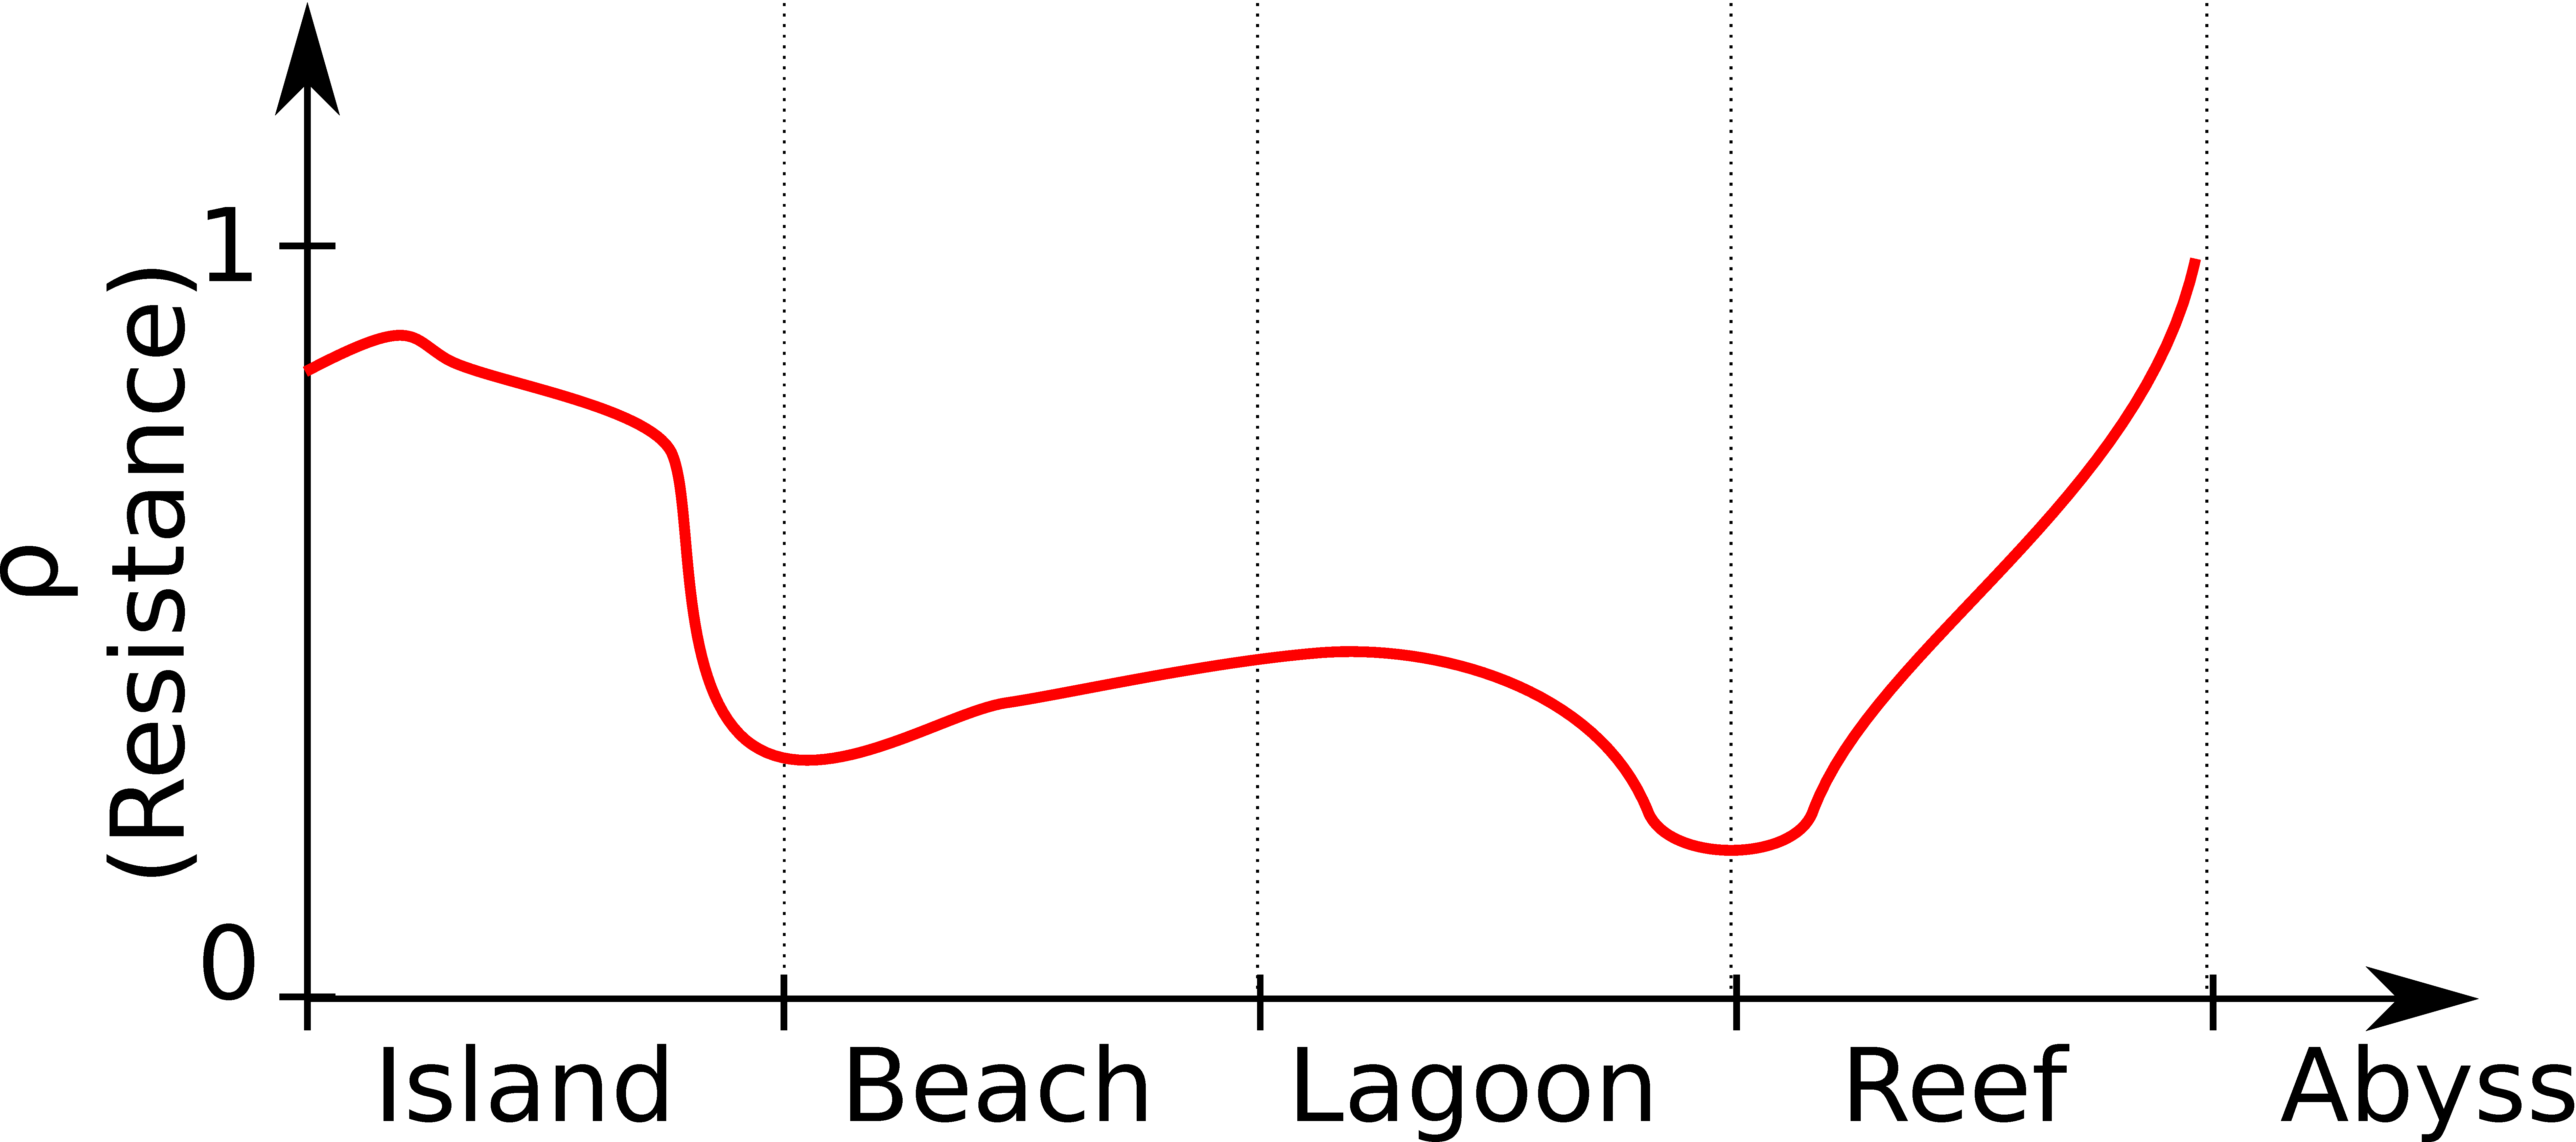
\includegraphics[width=0.45 \linewidth]{resistanceFunction.pdf}
%     \caption{The resistance function of the island is defined in the same way than the $\heightProfile$ function. The resistance to erosion and deformation arise from multiple factors such as depth, materials, wind shadowing, biotic and abiotic factors, ... Modeling all these factors is complex. As such, using a user-defined approximation through a resistance function $\resistance$ allows for more control. }
%     \label{fig:coral-island_resistance-function}
% \end{figure}



\subsection{Coral reef modeling}
\label{sec:coral-island_coral-reef}

Once the terrain has been generated and deformed by the wind, we simulate the long-term geological evolution of coral reef islands through two parallel processes: the subsidence of the volcanic island and the upward growth of coral reefs. As observed in nature, the volcanic base sinks over time while coral formations grow vertically to remain close to the water surface, following the “keep-up” strategy of reef development.

\subsubsection{Subsidence}
\label{sec:coral-island_subsidence}

Subsidence is modeled by uniformly scaling the original terrain height downward, simulating the gradual sinking of the volcanic landmass due to tectonic processes. The user specifies a subsidence rate $\subsidRate \in [0, 1]$, which controls how much the island has sunk. The subsided terrain is computed as:

\begin{align}
    \heightSubsid(\p) = (1 - \subsidRate) \cdot h_0(\p)
\end{align}

This factor is applied uniformly across the island, offering a geologically plausible and computationally efficient approximation of large-scale subsidence.

\subsubsection{Coral reef growth}
\label{sec:coral-island_reef-growth}

Coral reef growth is modeled independently from the subsiding terrain. The system generates a coral-specific height field $\heightCoral(\p)$ that remains near the sea surface regardless of the island's vertical shift, reflecting coral growth in biologically viable depth ranges (typically 0-30 meters below sea level).

\begin{figure}
    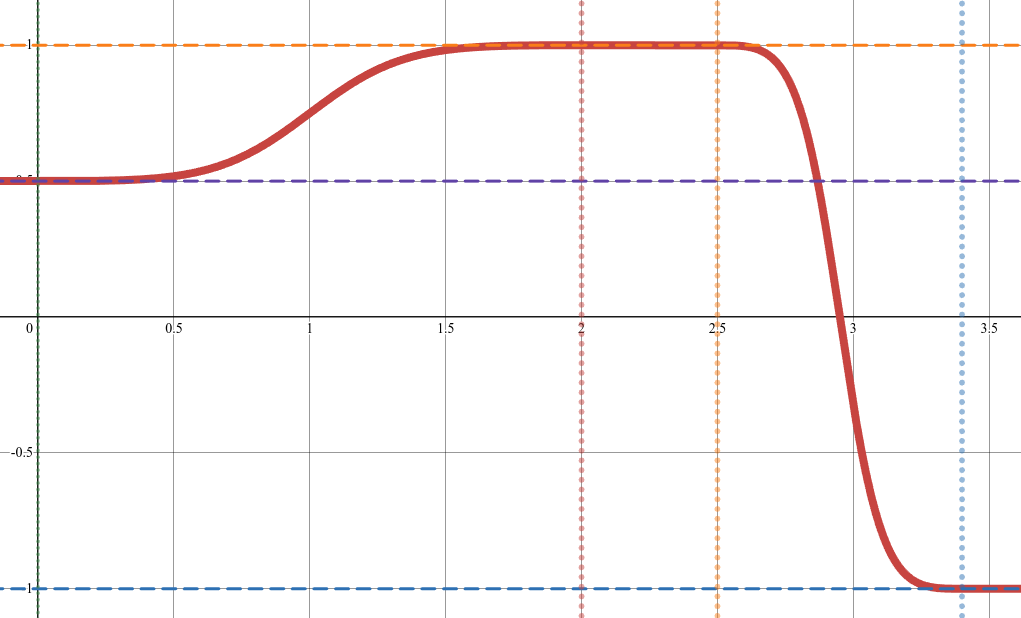
\includegraphics[width=0.7\linewidth]{Reef_function.png}
    \caption{The modeling of the reef growth in our model is described by a piecewise function $\heightCoral$ which is flat in the lagoon, the crest and abyss, and follows a smoothstep function as transitions for the backreef and fore reef regions. Zones' anchor heights are represented by horizontal dashed lines; zones' limits are dotted vertical lines. }
    \label{fig:coral-island_reef-function}
\end{figure}

We define distinct reef zones anchored at specific depths:
\begin{Itemize}
    \Item{} Reef crest near sea level: $h_\text{crest} = -2$\,m
    \Item{} Back reef and lagoon: $h_\text{back} = -20$\,m
    \Item{} Fore reef sloping to abyss: $h_\text{abyss} = -100$\,m
\end{Itemize}

Each reef subregion is defined over a parametric domain $x \in [0, 1]$. For instance:
\begin{Itemize}
    \Item{} Back reef: $x_{\text{back,start}} = 0$, $x_{\text{back,end}} = 0.5$
    \Item{} Reef crest: $x_{\text{crest,start}} = 0.75$, $x_{\text{crest,end}} = 0.8$
    \Item{} Abyss begins at $x_{\text{abyss,start}} = 1$
\end{Itemize}

We model transition zones between these regions using a smoothstep operator:
\begin{align}
    \smooth(x) = 3x^2 - 2x^3
\end{align}

We denote the interpolating function as:
\begin{align}
    S(a, b, x_0, x_1, x) = a + (b-a) \smooth\left(\frac{x - x_0}{x_1 - x_0}\right)
\end{align}

The complete coral height field, as displayed in \cref{fig:coral-island_reef-function}, is built as a piecewise function:
\begin{align}
    \heightCoral(x) &= \sum_{r \in \text{subregions}}{
    \begin{dcases}
        h_r & \text{if } x_{\text{r,start}} \leq x \leq x_{\text{r,end}} \\
        0 & \text{otherwise}
    \end{dcases}
    } \nonumber \\ 
    &+
    \sum_{t \in \text{transitions}} {
        \begin{dcases}
            S(h_{t}, h_{t+1}, x_{\text{t,end}}, x_{\text{t+1,start}}, x) & \text{if } x_{\text{t,end}} < x < x_{\text{t+1,start}} \\
            0 & \text{otherwise}
        \end{dcases}
    }
\end{align}



% \subsubsection{Blending height fields}
% \label{subsubsec:height-functions-blending}

% \begin{figure}
%     \autofitgraphics[]{blend_function_low_approx.png, blend_function_high_approx.png}
%     \autofitgraphics[]{blend_compare_closeup_low.png, blend_compare_closeup_high.png}
%     \caption{Blending two functions $f: \R \to \R$ (black) and $g: \R \to \R$ (blue) with the $\max$ operator (red), causing a discontinuity, and with the $\smoothmax$ operator (green), resolving the issue at the cost of slight underestimations with low values of $k$. Left: $k=5$, right: $k=50$}
%     \label{fig:coral-island_blend-function-island}
% \end{figure}

% \begin{figure}
%     \autofitgraphics[]{blend_function_with_upper_low.png, blend_function_with_upper_high.png}
%     \autofitgraphics[]{blend_closeup_k_5.png, blend_closeup_k_10.png, blend_closeup_k_50.png}
%     \caption{The $\smoothmax^+$ operator(orange) is a function that use to overestimate the maximum value of two functions, especially when the difference between the two functions is small, while the $\smoothmax^-$ function (green) tends to underestimate the $\max$ operator. Taking $\smoothmax$ (red) as the average of $\smoothmax^-$ and $\smoothmax^+$ creates a much more precise blending, even with lower values of $k$ (Left: $k=5$, center: $k=10$, right: $k=50$).}
%     \label{fig:coral-island_blend-function-island-with-upper}
% \end{figure}

% The final step is to blend the subsided height field $\heightSubsid(\p)$ with the coral feature height field $\heightCoral(\p)$ to produce the final terrain. The goal is to ensure that coral features remain near the water surface while allowing the rest of the island to subside.

% To achieve this, the system uses a smooth max function, which smoothly blends the two height fields. The smooth max function ensures that the coral regions dominate where coral growth is present, while the subsided island terrain dominates in other regions. This blending method ensures that the transition between the coral and subsided regions is smooth and visually consistent.

% We define our smooth max function $\smoothmax: a, b \in \R^2$ as the mean of two functions, $\smoothmax^-$ and $\smoothmax^+$, adapted from Ingo Quilez's smooth min function, that respectively underestimate and overestimate the function $\max$:

% \begin{align}
%     \smoothmax^-(a, b) &= a + \frac{b - a}{1 + \exp\left(-k \cdot (b - a) \right)} \\
%     \smoothmax^+(a, b) &= a + \frac{b - a}{1 - \exp\left(-k \cdot (b - a) \right)} \\
%     \smoothmax(a, b)   &= a + \frac{\smoothmax^-(a, b) + \smoothmax^+(a, b)}{2} %}{2}
% \end{align}

% Here, $a = \heightSubsid(\p)$ is the height from the subsided island, $b = \heightCoral(\p)$ is the height from the coral reef feature, and $k$ controls the smoothness of the transition. Higher values of $k$ brings the $\smoothmax$ function closer to the $\max$ function (\cref{fig:coral-island_blend-function-island}).

% This smooth max function guarantees visual continuity by preventing abrupt height differences between the coral regions and the subsided terrain, creating a smooth, gradual transition that mimics the natural blending of coral reefs with deeper areas. The coral feature height field takes precedence where coral can grow, typically in shallow regions. In deeper regions, such as the abyss, the subsided height field naturally dominates, ensuring that the final terrain accurately reflects both subsidence and coral growth processes.

% Note that the $\smoothmax$ function is undefined for $a = b$, however, a proof of continuity for $\smoothmax \in C^\infty$ is provided in \cref{chap:smoothmax-proof} resulting in:
% \begin{align}
%     \smoothmax(a, b) = \begin{dcases}
%         a + \frac{1}{2k} & \text{ if } a = b, \\
%         \frac{\smoothmax^-(a, b) + \smoothmax^+(a, b)}{2} & \text{otherwise}
%     \end{dcases}    
% \end{align}

\subsubsection{Output}
\label{sec:coral-island_procedural-output}

Finally, we merge the island base height field and the coral reef height field by our \textit{ad-hoc} smooth maximum operator $\smoothmax$ defined as:
\begin{align}
    \smoothmax(a, b) = \begin{dcases}
        % a + \frac{b - a}{2k} \left( \frac{1}{1+e^{-k(b - a)}} + \frac{1}{1-e^{-k(b-a)}} \right) &\text{for } a \neq b \\
        a + \frac{\delta}{2k} \left( \frac{1}{1+e^{-k\delta}} + \frac{1}{1-e^{-k\delta}} \right) &\text{for } a \neq b \\
        a + \frac{1}{2k} &\text{for } a = b
    \end{dcases}
\end{align} 
with $\delta=b-a$ for conciseness, and $k$ a sharpness parameter approximating the $\max$ operator as $k$ grows. At $k=5$, the operator $\max$ is already well approximated while conserving continuousness in the resulting height field $\height(p) = \smoothmax(\heightSubsid(\p), \heightCoral(\p))$.

The resulting terrain represents a plausible coral reef island, where the volcanic island has subsided, and coral reefs have grown upward to keep pace with the water level. The smooth blending between the subsided terrain and the coral features ensures a natural transition between regions like the island, lagoon, and coral reefs.

One of the key strengths of this method is its flexibility as the subsidence and coral reef growth processes are modeled independently, allowing for a wide range of configurations. Users can generate plausible island terrains with or without coral features, or apply the coral reef growth simulation to existing height fields from other sources.







\section{Training the cGAN}

In this section, we introduce the use of a conditional Generative Adversarial Network (cGAN), specifically the pix2pix model, to enhance the island generation process by increasing the variety and flexibility of terrains. While the initial procedural algorithm can create numerous island examples, cGAN provides additional flexibility in generating more complex terrain without the rigid constraints of the procedural algorithm that stem from our initial assumptions based on coral reef formation theory.

\subsection{Dataset generation}
\label{sec:coral-island_dataset-generation}


\begin{figure}
	\centering
	\autofitgraphics[]{examples-going-more-complex.pdf} %{placeholder.pdf}
    \caption{Using a large set of pairs of height field-label map, the training of a deep learning model result in a user-friendly interface requiring solely a hand-drawn label map to produce a 2.5D height field of the desired island.}
    \label{fig:coral-island_cGAN-pipeline}
\end{figure}


The creation of the dataset is done through the use of the procedural algorithm for which we alter the input parameters. 

For each generation, the top-view and profile-view sketches use an initial layout. Each outline of the top-view sketch is defined as a centered circle of random radius $\radius_\text{min} \leq \radius^* \leq \radius_\text{max}$. We add another deformation based on Perlin noise such that the final contour is defined as 
\begin{align}
    \radius(\angl) = \radius^* + \noise(\angl)
\end{align}

On the other hand, we define an initial profile-view sketch by defining $\heightProfile^*(\distRegions)$ the initial height function for which fBm noise is applied to obtain 
\begin{align}
    \heightProfile(\distRegions) = \heightProfile^*(\distRegions) \cdot \noise(\distRegions)
\end{align}

An identical process is done for the resistance function:
\begin{align}
    \resistance(\distRegions) = \resistance^*(\distRegions) \cdot \noise(\distRegions)
\end{align}

Finally, we need to generate a random wind field. The realistic nature of wind is ignored for the generation of the wind strokes in order to provide complexity and variety in the results. 
We generate a random number $n$ of strokes and their path by a uniformly sampling a random number $m$ of points. The spread and intensity of each stroke is also random.

Once all inputs are set, we generate an example for multiple level of subsidence $\subsidRate \in [0, 1]$ to obtain a height field incorporating the coral reef modeling and the associated label map. 

The Pix2pix model was originally pretrained using RGB images. In this training phase, the images were label using the HSV (Hue, Saturation, Value) color space, where the Hue component specifically carried the label information. Both the Saturation and Value components were kept neutral, meaning they did not convey any significant label-related data. The target images, the ones the model aimed to reproduce, were formatted in RGB.

For the purpose of fine-tuning the model, we retained the use of the Hue component to encode the labels from the label map. We introduced a new dimension to the model's learning capabilities by incorporating the subsidence rate, denoted as $\subsidRate$, into the Value component. This addition not only utilizes the model's existing capability to interpret the HSV format but also enriches the input data, which now carries additional, valuable environmental information.

Moreover, we purposefully left the Saturation component unchanged at this stage, reserving space for potentially including another parameter in the future, which would allow us to expand the model's utility without altering the foundational HSV encoding scheme established during its initial training. By adhering to this encoding format, we ensure continuity in data representation, which maximizes the efficiency of the pretrained model. This strategic update enhances the model's adaptability and broadens its applicability to tackle new, complex challenges more effectively.

This configuration allows the process to create quickly a large quantity of data, with multiple parameters, of a single island centered in the image. 

\subsection{Data augmentation}
\label{sec:coral-island_data-augmentation}

\begin{deferredfigure}
    \autofitgraphics[]{6_features.png, 6_heightmaps.png, 6_results.png}
    \caption{By applying our three data augmentation functions, the deep learning model learns to overcome some constraints previously set by the initial algorithm: (A) the translation removes the constraint to have an island ultimately at the center of the map, (B) the directional scaling, typical from image processing, reduces the symmety constraint on the results and (C) the copy-paste unlock the possibility to obtain more than one island per map.}
    \label{fig:coral-island_data-augmentation-examples}
\end{deferredfigure}

To enhance the variety of the dataset and improve the model's ability to generalize, we apply several data augmentation techniques:
\begin{Itemize}
    % \AltTextImage{
        \Item{Translation:} Since the original algorithm always centers the island, we translate the islands within the image to remove this constraint (\cref{fig:coral-island_data-augmentation-translation}). This ensures that the cGAN can generate islands in any position within the frame. 
        % }{translation_example.png}{}{fig:coral-island_data-augmentation-translation}

    % \AltTextImage{
        \Item{Directional scaling:} By scaling the terrain in one direction, we create elongated islands that resemble corridors or archipelagos, adding another layer of diversity to the dataset. Such islands are usually found on tectonic plates convergence boundaries, creating island arcs with high density of volcanic centers like the Izu-Bonin-Mariana arc system (\cref{fig:coral-island_data-augmentation-scaling} shows an example of elongated island). 
        % }{Babeldaob_island.png}{Babeldaob Island, in the Caroline Islands.}{fig:coral-island_data-augmentation-scaling}

    % \AltTextImage{
        \Item{Copy-paste:} In some cases, we combine multiple islands into a single sample, ensuring they do not overlap. The regions not covered by any island are assigned the abyss ID. Although this approach ensures non-overlapping regions, future work could explore using blending techniques to position islands more closely without the risk of overlap (\cref{fig:coral-island_data-augmentation-copy-paste}). 
        % }{copy_paste_example.png}{}{fig:coral-island_data-augmentation-copy-paste}
\end{Itemize}

All augmentation techniques are applied both to the height field and the label map simultaneously to ensure consistency between the input (the label map) and the output (the height field).







\section{Results and evaluation}

The resulting model for coral island generation enables a high control-level from a user perspective as the unconstraint painting allows for complex scenarios while producing in real-time the resulting height fields. In this chapter we used the software Blender to provide renders directly from the outputed height fields. As our pix2pix model is trained to output $256\times256$ images, the resolution of the 3D models is limited by this architecture.

\subsection{Control}
\label{sec:coral-island_control}

Using deep-learning-based models, most constraints from our initial assumptions are lifted (radial layout, isolated islands, ...). The control over the overall shapes of the islands regions are given through digital painting, here using the GIMP software. Each pixel of the image are encoded in HSV, with the region identifier encoded in the Hue channel. The user may increase or decrease the subsidence level of the island by modifying the Saturation channel over the whole image (see \cref{fig:coral-island_results-subsidence}).

Since the model is based on statistics over the pixel values instead of hard values, users are not limited to a finite number of region identifiers, meaning that the output is more or less robust to noise (due to image compression, for example) and to the fuzzy values resulting from anti-aliasing of brushes often set by default, or resizing algorithm, by image editors, or even due to compression algorithm. The example displayed in \cref{fig:coral-island_results-fuzzy} presents a sketch for which the outlines of the regions are at the same time blurry and with layouts that are not expected (such as the small red regions inside the southern lagoon region or the adjacency of beach regions directly with the abyssal region) on the top figure and over-saturated on the bottom figure. The learned model does not include inconsistancies and results in plausible 3D models.

The tolerence over the input values may be used to provide even more control about the transitions between two regions. \cref{fig:coral-island_results_dino} shows an example of input map with regions that are leaking over neighboring regions, and the introduction of new hue values non-existant in the dataset (light green and dark green) but are the interpolated hue value of mountain regions and beach regions.

Since the procedural phase included low randomness, the output of the cGAN is limiting its inpredictibility and the results to a slight change on the input create only slight changes on the output, preventing unexpected results. \cref{fig:coral-island_results-subsidence} shows the result of an input map with only a variation on the subsidence level, the resulting height fields are very similar. Adding the real-time computation of outputs, it becomes possible to construct progressively a landscape and correct small mistakes to intuitively design islands inspired by real-world regions (see an reproduction of Mayotte in \cref{fig:coral-island_example-Mayotte}). 


\begin{deferredfigure}
    \autofitgraphics[]{2_features.png, 2_heightmaps.png, 2_results.png}
    \autofitgraphics[]{1_features.png, 1_heightmaps.png, 1_results.png}
    \caption{An identical label map yield similar height fields over multiple inferences from the model, even after modifying the subsidence factor (visible in the luminosity of the input image).}
    \label{fig:coral-island_results-subsidence}
\end{deferredfigure}
\begin{deferredfigure}
    \autofitgraphics[]{3_features.png, 3_heightmaps.png, 3_results.png}
    \autofitgraphics[]{4_features.png, 4_heightmaps.png, 4_results.png}
    \caption{Using a generative neural network allows a higher level of tolerence on the user input. Here the user used an fuzzy brush to draw the label map, resulting in some pixels that are inconsistent with the dataset and unlogical island layouts (some small "abyss" regions [red] are found between "beach" [green], "lagoon" [cyan] and "reef" [blue]). The model ignores the inconsistencies even for over-saturated pixels. }
    \label{fig:coral-island_results-fuzzy}
\end{deferredfigure}
\begin{deferredfigure}
    \autofitgraphics[]{DinoIsland_features.png, DinoIsland_heightmaps.png, DinoIsland_results.png}
    \caption{Without constraints on the generation, the user may use unrealistic layout and the neural network will however output a plausible result.}
    \label{fig:coral-island_results_dino}
\end{deferredfigure}
\begin{deferredfigure}
    \autofitgraphics[]{Mayotte-example.png, 5_results.png}
    \caption{Comparison between of real (left) and synthetic (right) islands of Mayotte.}
    \label{fig:coral-island_example-Mayotte}
\end{deferredfigure}


\subsection{Performances}
\label{sec:coral-island_performances}

The Python script for the initial island dataset generation is poorly optimized and takes about 2.5s per island of size $256 \times 256$ as the parallelization does not take place here. Implementing an optimized C++ version of the initial generation process reduces this execution time to 50ms per generation.

On the other hand, the inference time for a single input image of dimension $256 \times 256$ is constant whatever the complexity of the scene. Using the NVIDIA GeForce GTX 1650 Ti GPU with Python 3.10 and PyTorch version 2.5.1+cu121, the inference time measured is 5ms (std 1.1ms). 

We not only show that using a neural network reduces the constraints on the generation process, but also that the execution time is only dependant on the network architecture, without influence from the dataset generation algorithm. 








% \section{Advantages, limitations, and future works}


% One of the main strengths of this approach is its ability to produce a wide variety of island terrains, even in the absence of real-world data. The procedural generation methods allow for high flexibility in designing both the shape and features of the island, while the use of cGAN enables further refinement and the generation of terrains that are not bound by the original constraints of the procedural model. By combining these two methods, we leverage the advantages of both: the structured control of procedural techniques and the pattern-learning capabilities of deep learning.

% A key advantage of this approach is the retention of semantic information about the terrain throughout the generation process. The label map, which serves as the input to the cGAN, can also be used after terrain generation to provide a detailed representation of the different regions of the island (such as the beach, lagoon, coral reef, and island body). This label map can guide post-processing operations, such as applying different textures based on terrain features or adding other environmental elements like vegetation. The preservation of semantic information provides a useful connection to the next stage of terrain manipulation, making the process more versatile and adaptable to different use cases.

% Furthermore, the use of an out-of-the-box cGAN model highlights the feasibility of employing existing neural network architectures with minimal modifications in the field of procedural generation. This is particularly important in domains where real-world data is scarce, such as coral reef islands, allowing synthetic data to be effectively used for training purposes.

\begin{deferredfigure}
    \autofitgraphics[]{random-input-2.png, random-height-2.png, random-render-2.png}
    \autofitgraphics[]{random-input-1.png, random-height-1.png, random-render-1.png}
    \autofitgraphics[]{random-input-3.png, random-height-3.png, random-render-3.png}
    \autofitgraphics[]{random-input-4.png, random-height-4.png, random-render-4.png}
    \caption{Starting from random Perlin noise, transformed into a label map, we can generate a large variety of results. }
    \label{fig:coral-island_perlin-examples}
\end{deferredfigure}




% While the cGAN model provides increased flexibility and variety in island generation, it does come with certain limitations:

% \begin{Itemize}
%     \Item{Biases from the synthetic dataset:} Since the cGAN model is trained entirely on a procedurally generated dataset, it inherits the biases present in the initial algorithm. For example, while the model can break free from the radial symmetry constraint and center positioning, it still relies on the synthetic data's structure and patterns. This can limit the true diversity of the generated terrains, as the cGAN cannot generate terrains that deviate too far from the examples in the training set.
%     \Item{Lack of user control:} Another limitation of using cGAN in this context is the lack of real-time user control during terrain generation. While traditional procedural generation methods allow users to tweak parameters (e.g., island size, beach width) during the generation process, the cGAN model operation is abstracted from the user, providing no mechanism for direct interaction beyond the initial label map. This reduces the level of customization available to the user.
%     \Item{Data-driven dependence:} The quality of the generated terrain depends entirely on the quality of the training dataset. Since the dataset is synthetically generated, any limitations or biases in the initial dataset directly affect the cGAN's output. This dependence on data quality makes it crucial to design a well-augmented and varied dataset to ensure diverse and realistic outputs.
% \end{Itemize}

% While this approach brings significant advantages, there are also some limitations to consider. The reliance on a synthetic dataset means that the cGAN inherits some biases and limitations of the original procedural algorithm. This could limit the true diversity of the terrains that the model can generate, as the output is confined by the patterns present in the training data. Additionally, the cGAN model's internal logic lacks transparency, offering limited user control over the generation process once the model has been trained. This contrasts with traditional procedural methods, which typically allow for real-time tweaking of parameters.


\section{Conclusion and future work}

This work has presented a novel approach to generating coral reef island terrains by combining traditional procedural methods with deep learning techniques. We first developed a procedural generation algorithm capable of creating a wide variety of island terrains through a combination of top-view and profile-view sketches, wind deformation, and subsidence and coral reef growth simulation. By applying these methods, we were able to produce realistic terrains based on geological processes, capturing key features of coral reef islands such as beaches, lagoons, and coral reefs.

To further enhance flexibility and realism in the generation process, we incorporated a Conditional Generative Adversarial Network (cGAN), using the pix2pix model to generate height maps from label maps of island features. The cGAN model allowed us to overcome some of the constraints inherent in the procedural algorithm, such as radial symmetry and fixed island positioning. With data augmentation techniques, we were able to train the cGAN on a synthetic dataset, generating varied and realistic island terrains.

\paragraph{Limitations} 
While this approach brings significant advantages, there are also some limitations to consider. The reliance on a synthetic dataset means that the cGAN inherits some biases and limitations of the original procedural algorithm. This could limit the true diversity of the terrains that the model can generate, as the output is confined by the patterns present in the training data. Additionally, the cGAN model's internal logic lacks transparency, offering limited user control over the generation process once the model has been trained. This contrasts with traditional procedural methods, which typically allow for real-time tweaking of parameters.

\paragraph{Future work}
Further improvements could be made to the synthetic dataset. Incorporating more complex geological processes, such as wave erosion or tidal influences, could lead to even more realistic terrains. Additionally, refining the way islands are blended in multi-island samples, or adding more diverse input conditions (e.g., different geological settings), could help the model generalize better and produce more varied and dynamic landscapes.  While the current model allows for rapid terrain generation, adding more options for users to interact with the cGAN, such as tweaking parameters like wind strength or island size, could enhance the flexibility of the system. 
Many other neural networks models could be exploited to increase the possibilities, such as newer variants of cGANs \cite{Park2019}, or models with style transfer functionalities \cite{Gatys2015,Zhu2020} in order to change the overall aspect of a terrain \cite{Perche2023a,Perche2023b}, use text-to-images models \cite{Rombach2021,Radford2021} to generate height fields from a verbal prompt, or super-resolution models \cite{Dong2014} to increase the definition of details in the final output \cite{Guerin2016a}.


% There are several directions for future research and improvements. One promising avenue is to incorporate the wind velocity field more directly into the cGAN training process, potentially as an additional input condition. This would allow the model to better capture wind-driven terrain features such as cliffs or other deformations influenced by wind patterns.

% Another area for exploration is improving user interaction during the terrain generation process. While the current model allows for rapid terrain generation, adding more options for users to interact with the cGAN, such as tweaking parameters like wind strength or island size, could enhance the flexibility of the system.

% Finally, further improvements could be made to the synthetic dataset. Incorporating more complex geological processes, such as wave erosion or tidal influences, could lead to even more realistic terrains. Additionally, refining the way islands are blended in multi-island samples, or adding more diverse input conditions (e.g., different geological settings), could help the model generalize better and produce more varied and dynamic landscapes.


% One possible future improvement could involve incorporating the wind velocity field into the cGAN training process. While the label map is the only input used in the current implementation, the wind field could be added as an additional condition. This would be especially useful if the initial algorithm were augmented to include wind-driven features, such as cliffs or specific terrain deformations influenced by wind patterns. Adding the wind field as an input could help the cGAN generate more realistic terrains that better reflect the influence of wind on the landscape.

% Additionally, further development could explore improving how multiple islands are combined in a single sample. For example, using blending techniques to handle overlapping regions could allow islands to be positioned closer together, enabling the generation of more complex archipelagos without sacrificing the integrity of the height field.

% Many other neural networks models could be exploited to increase the possibilities, such as newer variants of cGANs \cite{Park2019}, or models with style transfer functionalities \cite{Gatys2015,Zhu2020} in order to change the overall aspect of a terrain \cite{Perche2023a,Perche2023b}, use text-to-images models \cite{Rombach2021,Radford2021} to generate height fields from a verbal prompt, or super-resolution models \cite{Dong2014} to increase the definition of details in the final output \cite{Guerin2016a}.

% \bibliographystyle{eg-alpha-doi}
% \bibliography{egbibsample}
\printbibliography[title=References]

\clearpage
\deferredfloats

\end{document}